\documentclass[12pt, oneside]{article}   	                 		
\usepackage{graphicx}
\usepackage{epstopdf}
\usepackage{cite}
\usepackage{setspace}
\usepackage{mathtools}
\usepackage{amsmath}
\usepackage{amssymb}
\usepackage{caption}
\usepackage{subcaption}
\usepackage{tabularx}
\usepackage{fullpage}  
\usepackage{enumerate}
\usepackage{enumitem}
\setlist{nolistsep}
\usepackage{url} 
\usepackage{multicol}
\usepackage{appendix}
\usepackage[section]{placeins}
\usepackage{morefloats}
\usepackage{topcapt}
\usepackage{graphicx}
\graphicspath{{/home/wwwennie/wwwennie@gmail.com/UT-Austin/teaching/Elective-Computational-Methods-MatSci/projects/4-MDSurf/figs/}}

\title{CHE384T Pset 4: Molecular dynamics}
\author{Solutions}

\begin{document}
\maketitle

Included is the code that was used in this problem set. Due to the fact that several modifications were made to each of the files, the relevant files of code are listed specifically to each problem where appropriate. All runs and plots of graphs are located in the corresponding \verb!PS4-*.py!.


%--------------------------------------------------------------------------------%
\section{Exercise 1: One Atom on the Surface}

To simulate on atom on the surface, we use the Verlet algorithm and a surface potential of the form

\begin{equation}
     \phi (x,y) = A sin(\pi x)sin(\pi y)
\end{equation}

Since we deal with one atom, we input the energy. No periodic boundary conditions are used. For this exercise, we use the given and constructed files 

\vspace{5mm}
 \begin{enumerate}
   \item \verb!initsurf.py!   $\rightarrow$ initialization of positions and velocities.
   \item \verb!phisurf.py!  $\rightarrow$ contains surface potential.
    \item \verb!fsurf.py!     $\rightarrow$ contains corresponding force of \verb!phisurf.py!.
    \item \verb!MDSurf.py!  $\rightarrow$ contains implementation of Verlet Algorithm for one atom on 2D surface.
    \item \verb!averaging.py!  $\rightarrow$ gives thermodynamic averages of energies, temperature, and pressure.
\end{enumerate}
 \vspace{5mm}

\subsection{Time step for numerical error}
We first find the appropriate time step that preserves conservation of energy. In Figure \ref{fig:atomdt}, we show two different time step intervals and the corresponding energy. We use A = $E_{in}$ = 1.

To determine whether our chosen parameters result in the conservation in energy, we examine the fluctuations of total energy. Using the criteria that $\frac{E_{max}-E_{min}}{<E>} ~ 10^{-4} $, we choose dt = 0.006 in reduced units. 

\begin{figure}
\begin{minipage}[!htbp]{.49\linewidth}
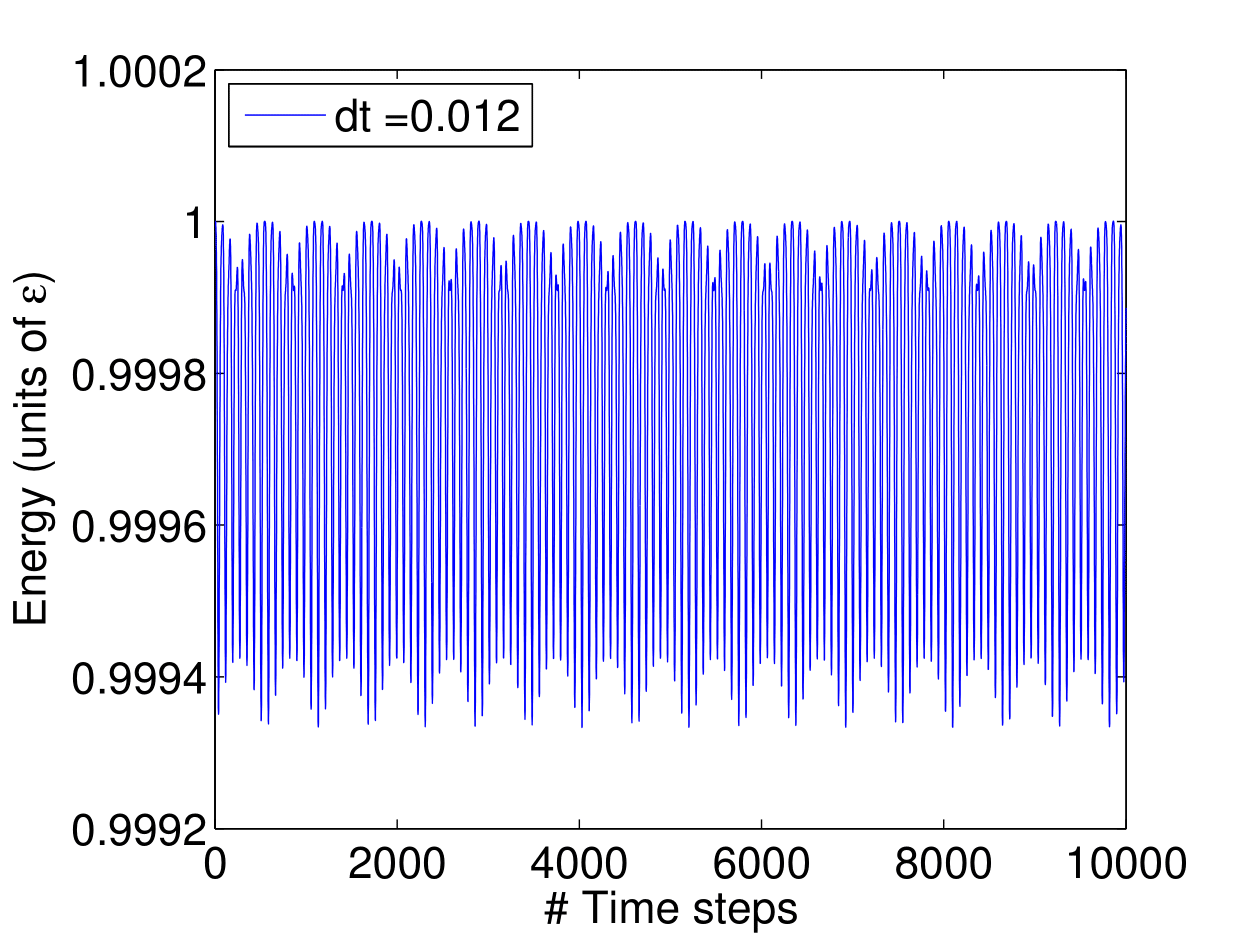
\includegraphics[width=\textwidth]{./figs/ex1a-1.png}
\end{minipage}
\begin{minipage}[!htbp]{.49\linewidth}
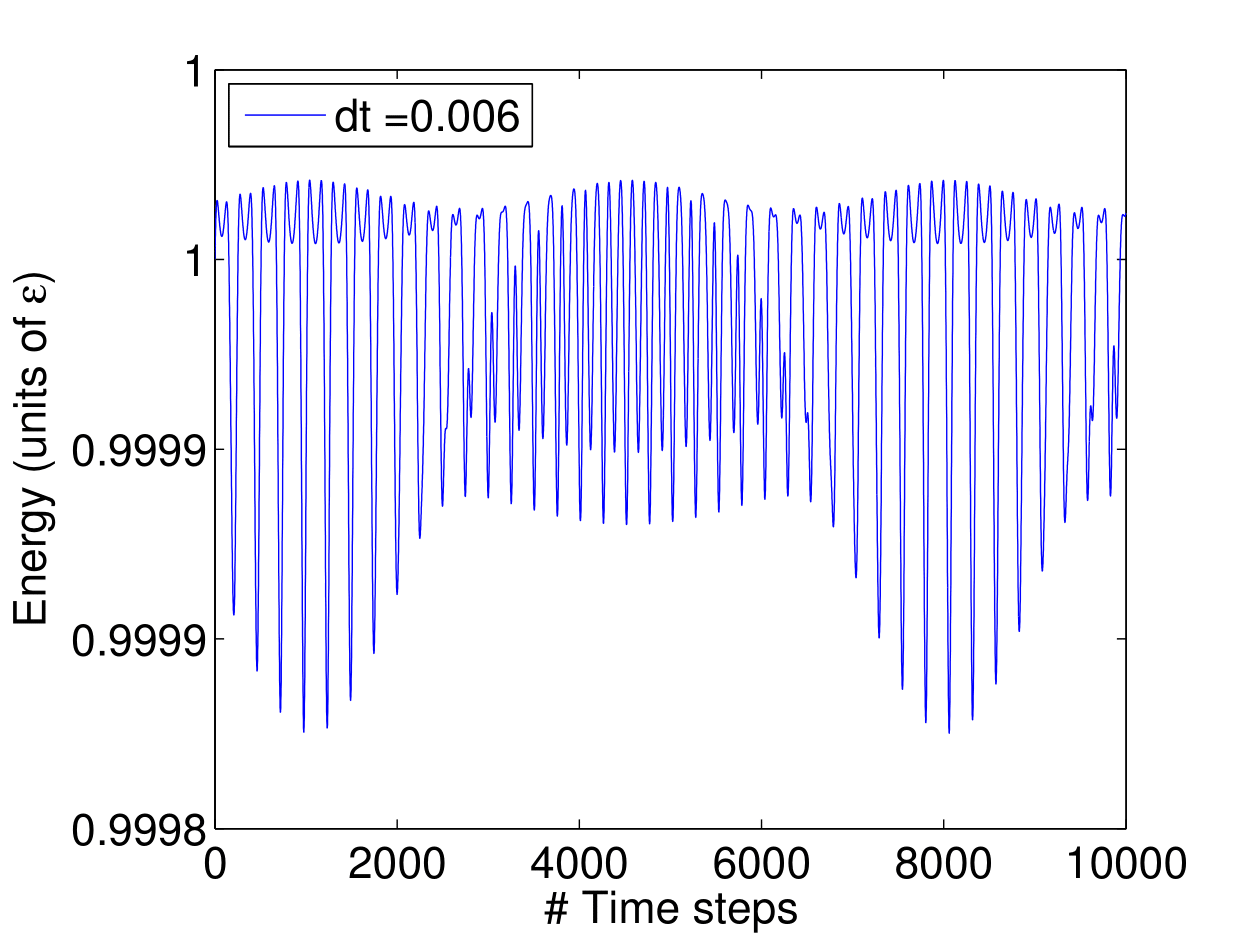
\includegraphics[width=\textwidth]{./figs/ex1a-2.png}
\end{minipage}
\caption{Convergence of fluctuations in total energy for varying time steps in reduced units, (a) dt = 0.012 and (b) dt = 0.006}
\label{fig:atomdt}
\end{figure}

\subsection{Varying E}

We next vary the inputed energy to examine the behavior between the total, potential, and kinetic energy. As seen in Figure \ref{fig:varye}, the total energy remains constant (fluctuations are small compared to the axes plotted). In contrast, the kinetic and potential energy fluctuate noticeably. Increases in kinetic energy correspond to decreases in potential energy, and vice versa, reflecting the harmonic oscillator like behavior of the particle on the surface. All runs were done with 5000 time steps.

\begin{figure}
\begin{minipage}[!htbp]{.5\linewidth}
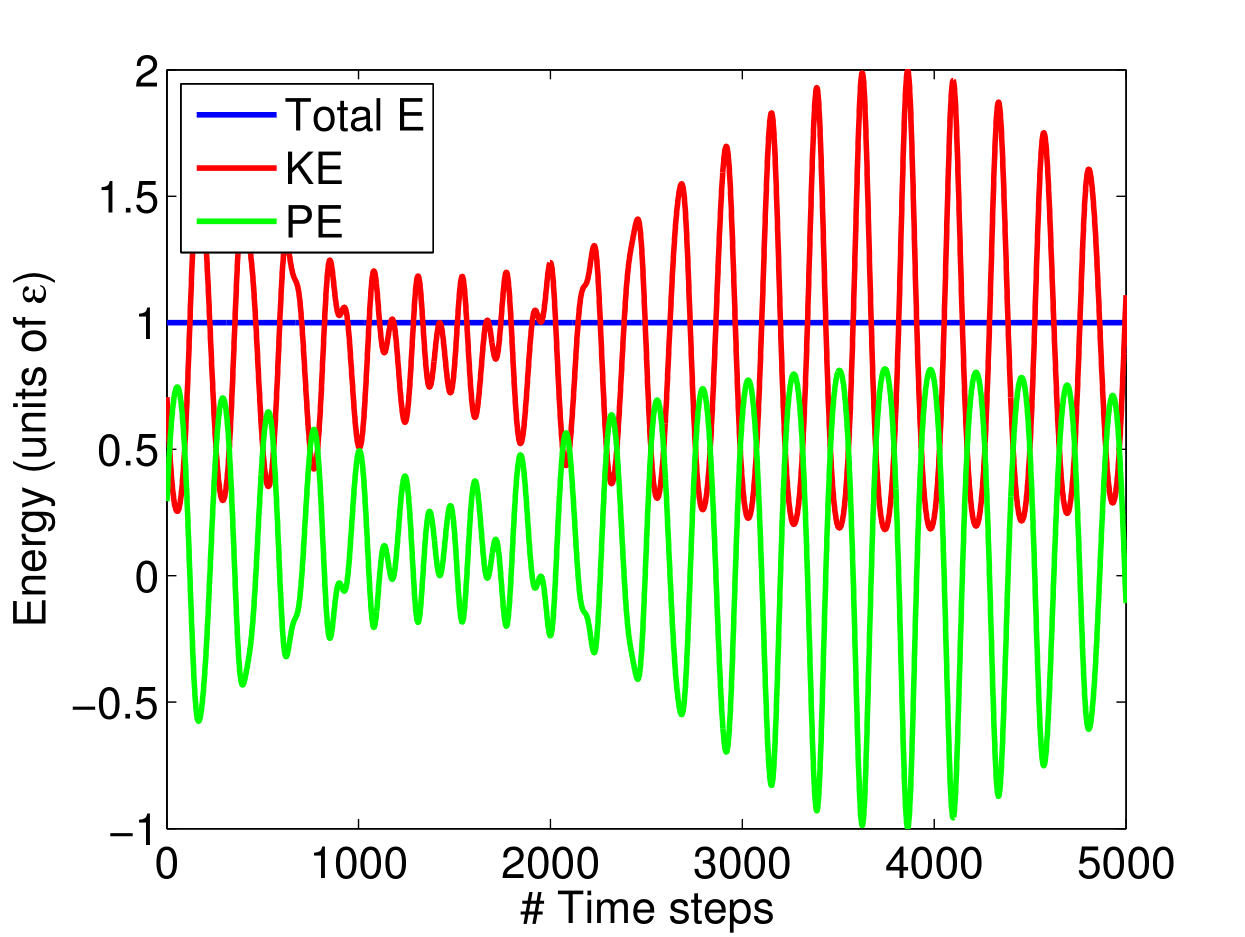
\includegraphics[width=\textwidth]{./figs/ex1b-e=1.png}
\subcaption{}
\end{minipage}
\hspace{0.02\linewidth}
\begin{minipage}[!htbp]{.5\linewidth}
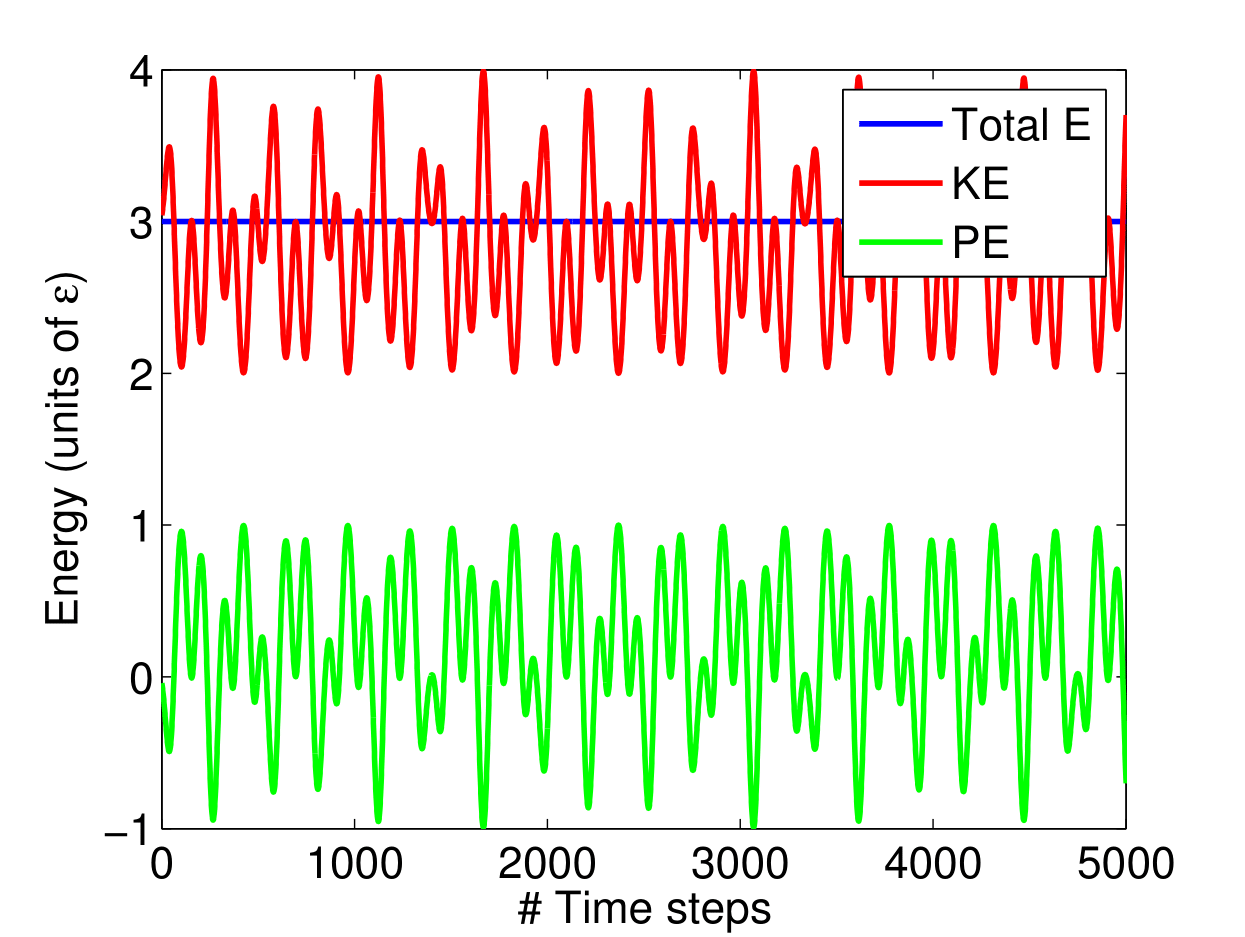
\includegraphics[width=\textwidth]{./figs/ex1b-e=3.png}
\subcaption{}
\end{minipage}
\hspace{0.02\linewidth}
\begin{minipage}[!htbp]{.5\linewidth}
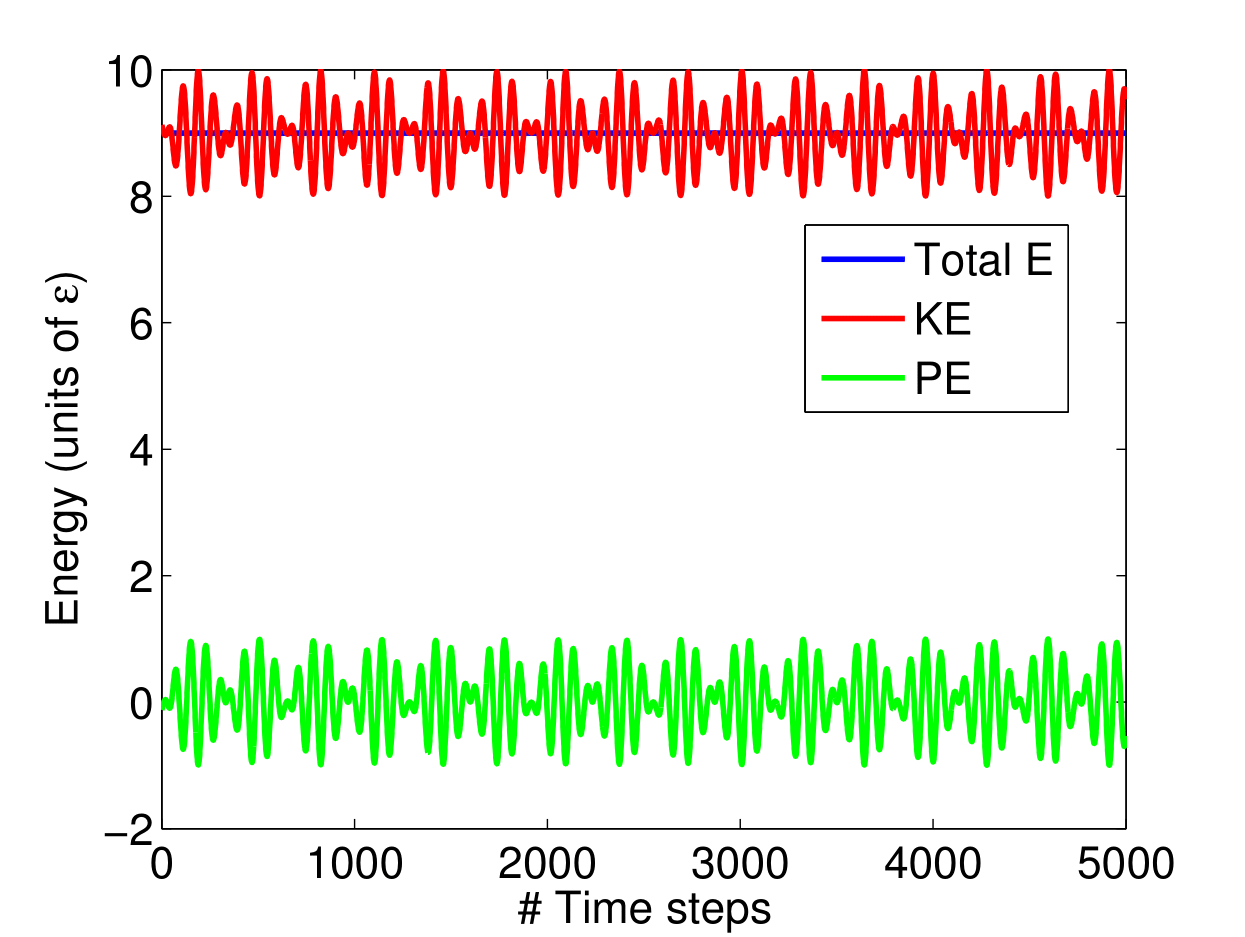
\includegraphics[width=\textwidth]{./figs/ex1b-e=10.png}
\subcaption{}
\end{minipage}
\caption{Tracking the relation between total, potential, and kinetic energy of one atom on a surface potential for (a) $E_{in} = 1$, (b) $E_{in} = 3$, and (c) $E_{in} = 10$ with 5,000 time steps; units of energy are in reduced units.}
\label{fig:varye}
\end{figure}

\subsection{$<u>$ and $<K>$}

We additionally report the average potential and kinetic energies for the one atom system on a surface potential. The below numbers are for 20,000 steps, dt = 0.006, A = 4, and $E_{in}$ = 1. The averages are done not including the first 200 time steps to exclude any time for equilibration.   

\begin{verbatim}
au = -1.0779
ak = 2.0778
ae = 0.9999   % for comparison to
\end{verbatim}

The kinetic energy is directly proportional to the temperature, by the equipartition theorem. For a two dimensional system consisting of one atom, $K = k_b T$, where $k_b$ is Boltzmann's constant.

\subsection{Atom motion and energy, and corresponding trajectory}

As the parameters for the potential surface remain constant, the fraction of potential energy of the total energy diminishes with increasing $E_{in}$. The strength of interaction with the surface potential is directly proportional to $A$. For convenience, we choose A = 1. The atom is initialized to be in a well near the origin.

For sufficiently high $E_{in} > A$, we would expect that on average the particle has enough kinetic energy to move nearly uninhibited by the surface potential. In contrast, for $E_{in} < A$, the particle has less available kinetic energy, and thus would have a much shorter net trajectory. This is indeed what is observed in Figure \ref{fig:traj}. For comparison, $E_{in} \approx A$ is also plotted, and exhibits a trajectory intermediate to the two extreme aforementioned cases. 

For $E_{in} = 0.1 < A $, the particle essentially stays in the well it was initialized in and is essentially stationary, as it does not have sufficient kinetic energy to escape the well. In contrast, the atom with $E_{in} = 5 > A$ is able to pass through the potential with the initial velocity with little problem, as if potential were a small perturbation. The intermediate case shows a combination of both behaviors, in which the trajectory of the the particle is clearly altered by the potential, but not sufficiently so that it halts its motion across the surface.

\begin{figure}
\begin{minipage}[!htbp]{.5\linewidth}
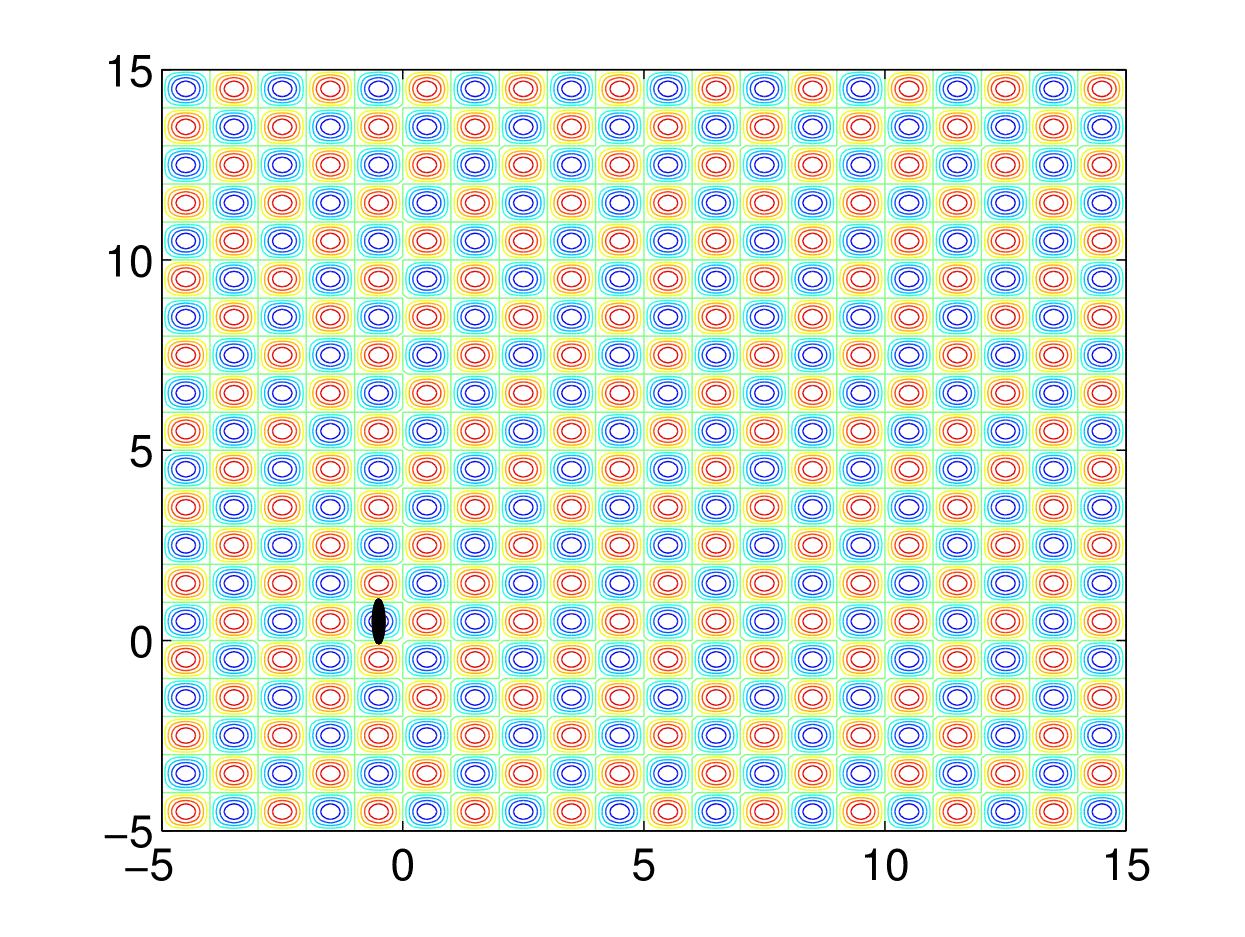
\includegraphics[width=\textwidth]{./figs/ex1e-e=p1.png}
\subcaption{}
\end{minipage}
\hspace{0.02\linewidth}
\begin{minipage}[!htbp]{.5\linewidth}
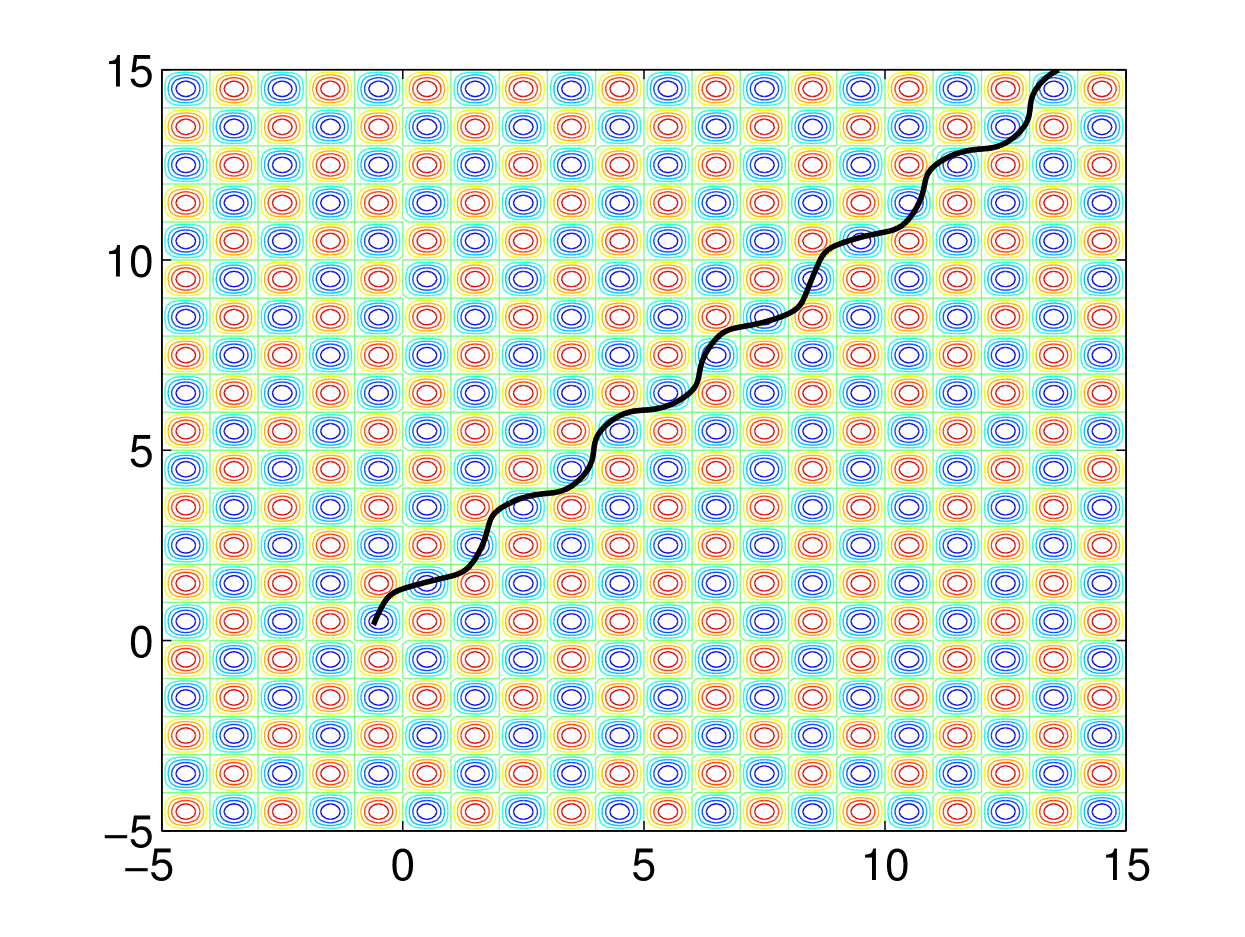
\includegraphics[width=\textwidth]{./figs/ex1e-e=1.png}
\subcaption{}
\end{minipage}
\hspace{0.02\linewidth}
\begin{minipage}[!htbp]{.5\linewidth}
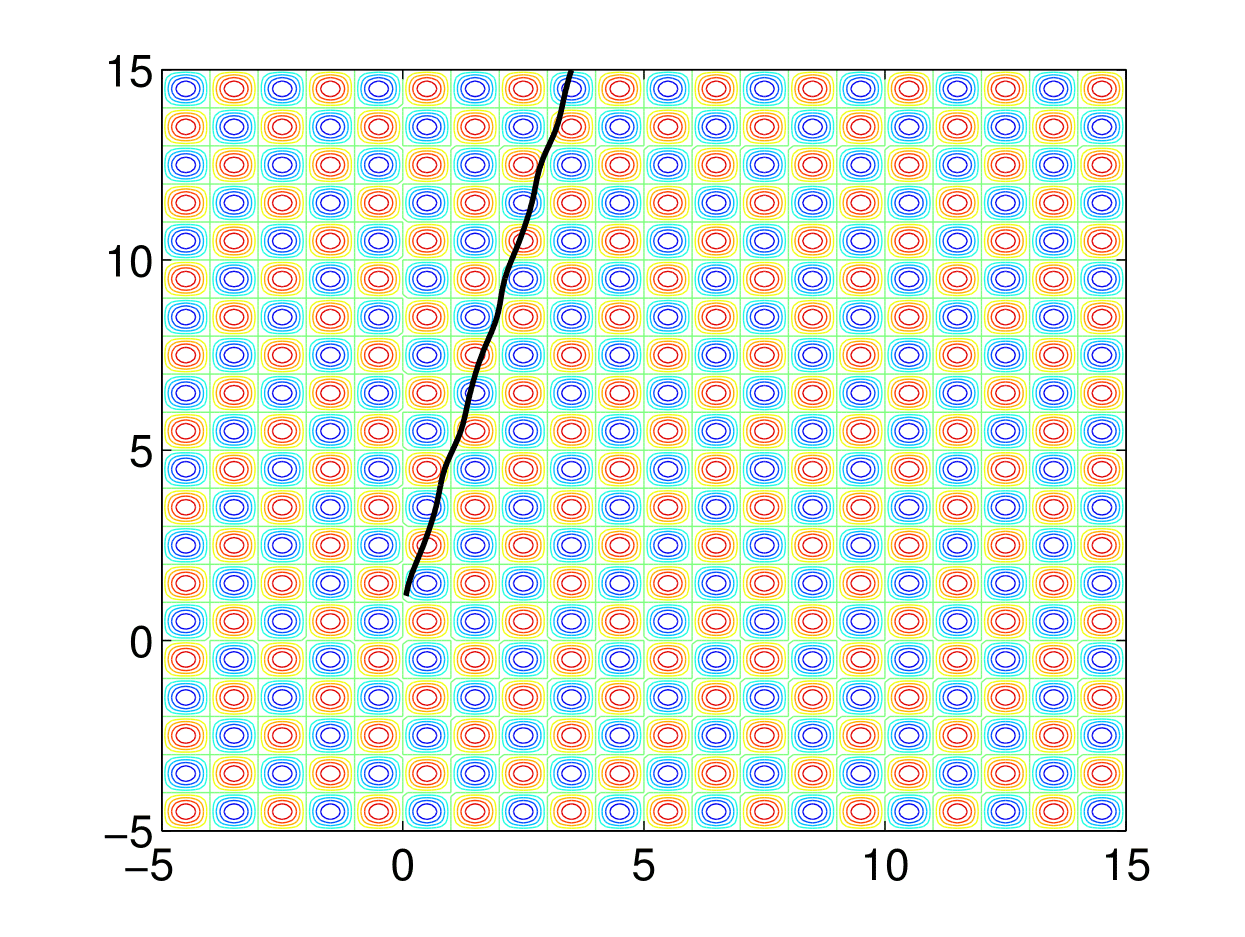
\includegraphics[width=\textwidth]{./figs/ex1e-e=5.png}
\subcaption{}
\end{minipage}
\caption{Trajectory of one atom on contour of surface potential for (a) $E_{in} = 0.1$, (b) $E_{in} = 1$, and (c) $E_{in} = 5$ for A = 1 with 10,000 time steps; units of energy are in reduced units.}
\label{fig:traj}
\end{figure}

%--------------------------------------------------------------------------------%
\section{Exercise 2: Multiple Atoms on the Surface}

Now we add additional atoms and interactions between them using the Lennard-Jones potential. For this exercise, the following files were used

\vspace{5mm}
 \begin{enumerate}
   \item \verb!initsurf2.py!   $\rightarrow$ initialization of positions of \textit{n} atoms; atoms are randomly placed in a well an then slightly displaced randomly in that well; initialization occurs such that no more than one atom sits in a well.
   \item \verb!MBinit.py!   $\rightarrow$ initialization of velocities for \textit{n} atoms in Maxwell-Boltzmann distribution centered around zero based off of desired temperature input.
   \item \verb!phisurf.py!  $\rightarrow$ contains surface potential.
    \item \verb!fsurf.py!     $\rightarrow$ contains corresponding force of \verb!phisurf.py!.
     \item \verb!fLJ2.py!     $\rightarrow$ contains calculation of forces for 2D Lennard-Jones system; also outputs corresponding potential energy.
    \item \verb!MDSurfLJ.py!  $\rightarrow$ contains implementation of Verlet Algorithm for one atom on 2D surface and interaction using Lennard-Jones potential.
    \item \verb!averaging.py!  $\rightarrow$ gives thermodynamic averages of energies, temperature, and pressure.
\end{enumerate}
 \vspace{5mm}
 
Figure \ref{fig:init} gives an example initial configuration for 10 atoms, as implemented by \verb!initsurf2.py!.

\begin{figure}[htbp]
   \centering
   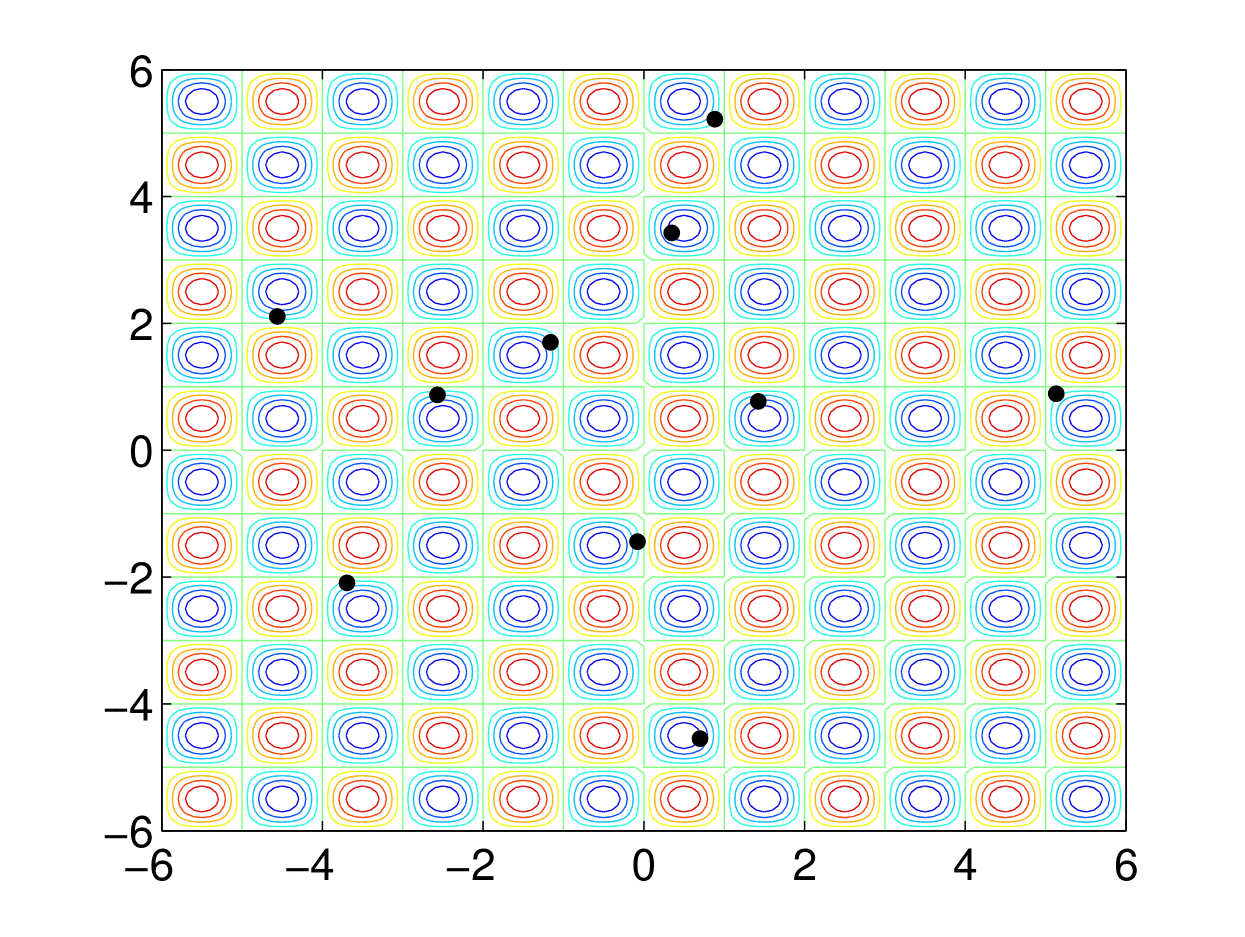
\includegraphics[width=0.5\textwidth]{./figs/ex2-init.png} % requires the graphicx package
   \caption{Example initial position configuration for modeling multiple atoms on 2D surface potential with Lennard-Jones interactions}
   \label{fig:init}
\end{figure}

Since we invoke the minimum image convention, we must rescale the positions of atoms that have trajectories outside the 6 x 6 simulation cell with lattice constant of unity we have chosen. This is implemented in \verb!PS4-*.py!, which determines how much the trajectory of each atom folds upon itself in the simulation cell. That is, if the trajectory of the atom leaves the top of the cell, it is observed to continue from the bottom of the cell.

In Figure \ref{fig:trajmult} we plot the trajectories for a system of 4 atoms over 3,000 time steps for dt = 0.006. A similar behavior is observed as with the one atom system. Instead of inputting energy, we input temperature, which determines the statistical distribution of velocities of the atoms in the system. When $T_{in}$ is comparable to A, there is observed clustering of the atoms, as seen by the fact that few trajectories in the upper half of the simulation cell, but also some interaction and spread in motion. Likewise, when the kinetic energy, proportional to $T_{in}$ is much smaller than A, there is insufficient kinetic energy, and so the atoms remain in their respective wells; the surface potential dominates the interactions. Finally, when $T_{in}$ is larger than A, there is more available kinetic energy. Limited clustering is observed, but the particles act more like non-interacting particles with high kinetic energies, as seen by the large spread of trajectories in the plot. 

\begin{figure}
\begin{minipage}[!htbp]{.5\linewidth}
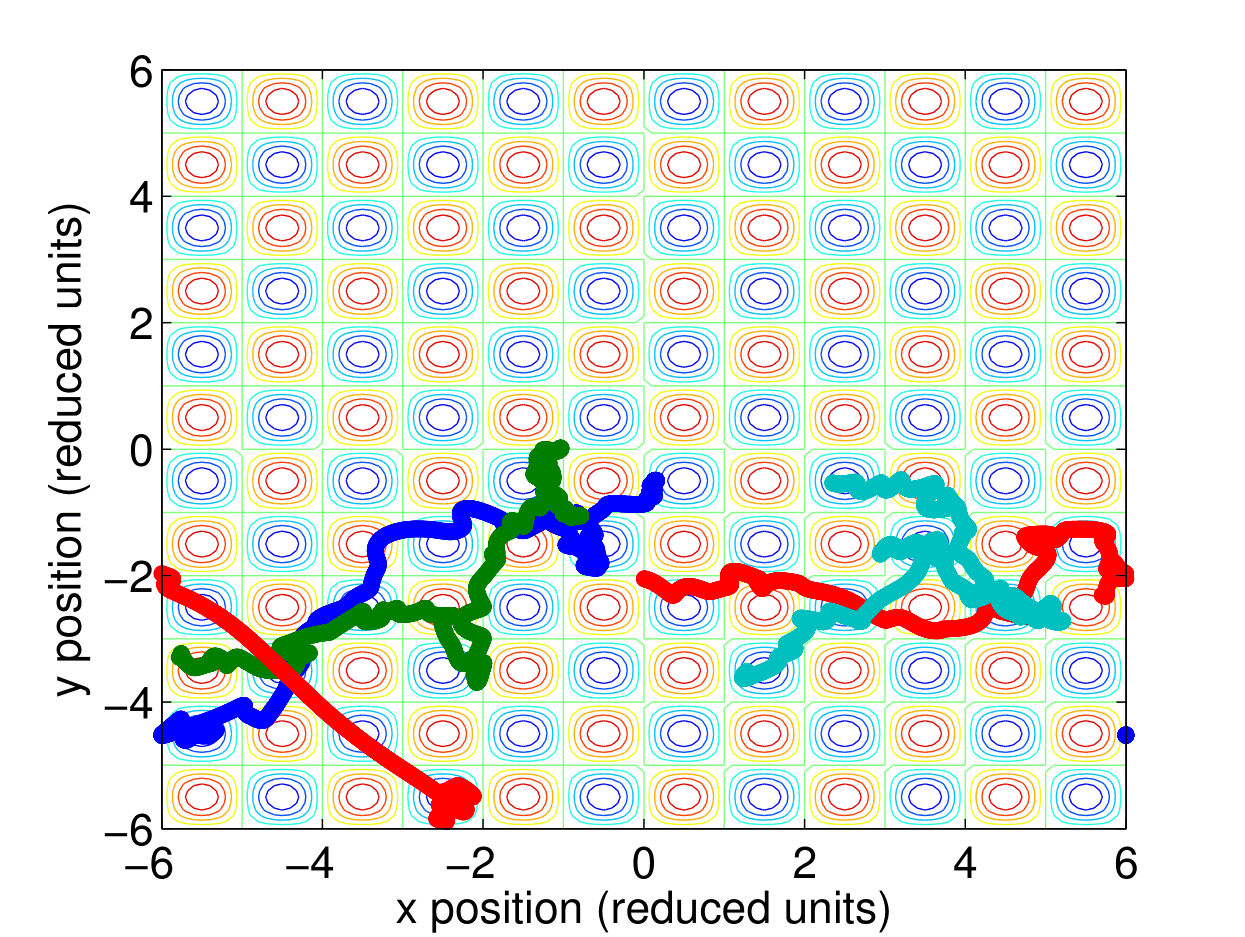
\includegraphics[width=\textwidth]{./figs/ex2-4n-acon0p1-tin0p1-3e3.png}
\subcaption{}
\end{minipage}
\hspace{0.02\linewidth}
\begin{minipage}[!htbp]{.5\linewidth}
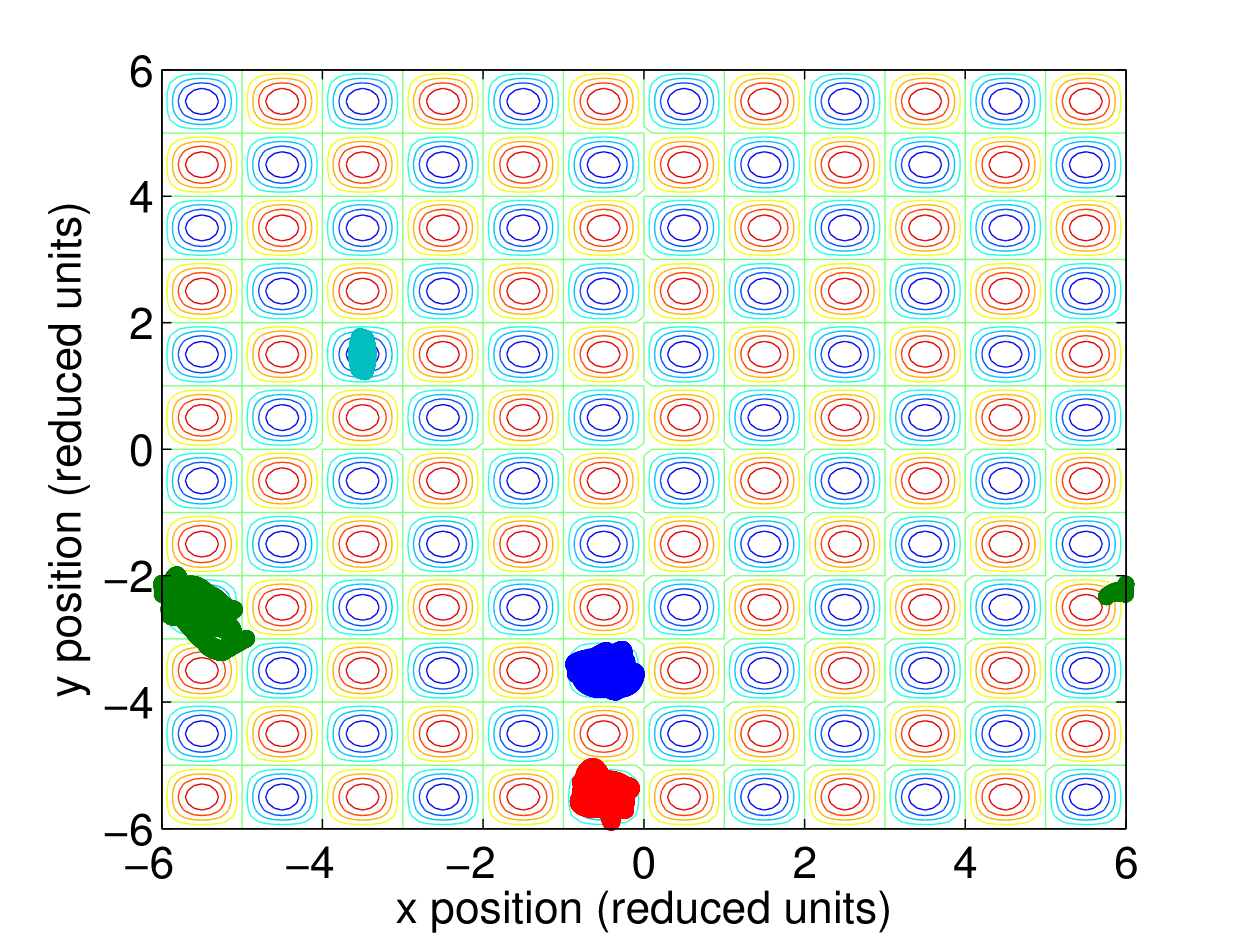
\includegraphics[width=\textwidth]{./figs/ex2-4n-acon1-tin0p1-3e3.png}
\subcaption{}
\end{minipage}
\hspace{0.02\linewidth}
\begin{minipage}[!htbp]{.5\linewidth}
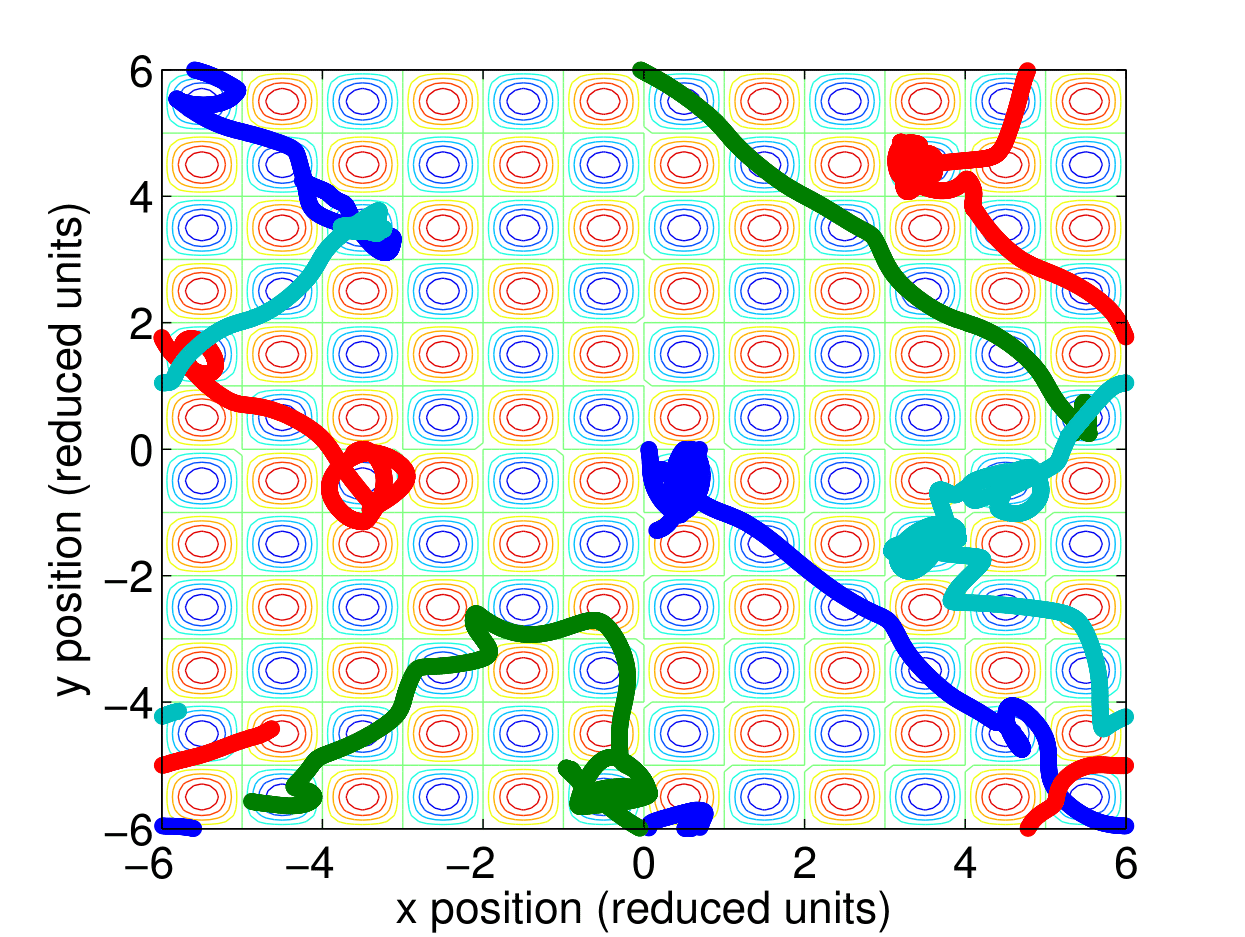
\includegraphics[width=\textwidth]{./figs/ex2-4n-acon1-tin1p2-3e3.png}
\subcaption{}
\end{minipage}
\caption{Trajectory for four atoms on contour of surface potential for (a) $T_{in} = A = 0.1$, (b) $T_{in} = 0.1, A = 1$, and (c) $T_{in} = 1.2, A = 1$ for 3,000 time steps; all quantities are in reduced units.}
\label{fig:trajmult}
\end{figure}

%--------------------------------------------------------------------------------%
\section{Exercise 3: Even More Atoms on the surface}

We repeat our above analysis for a different density of atoms on the surface. Here we choose to model a system of 10 atoms on our 6 x 6 simulation cell with lattice constant of unity.

When $T_{in}$ is comparable to A, there is observed but limited clustering of the atoms. That is, there is a fair spread of trajectories and interaction between atoms, as seen by the squiggly trajectories. Indeed, unlike the four atom case, there is much more wiggle to the trajectories indicating the increased influence of atomic interactions from the Lennard-Jones potential. For the case when the kinetic energy, proportional to $T_{in}$ is much smaller than A, there is insufficient kinetic energy, and so the atoms remain in their respective wells; the surface potential dominates the interactions, as was found in the four atom case. There is more variation to the motion of the atoms in their respective wells, as there is more variation in the initial velocities possible Finally, when $T_{in}$ is larger than A, there is more available kinetic energy. Limited clustering is observed, but the particles act more like non-interacting particles with high kinetic energies, as seen by the large spread of trajectories in the plot and that some atoms are able to traverse quite far in the simulation cell without being deflected significantly. 

It is worth noting that it is possible for such a small density of atoms, that extremely large velocities may be initialized, especially as the choice of initial total momentum of the system is zero.

\begin{figure}
\begin{minipage}[!htbp]{.5\linewidth}
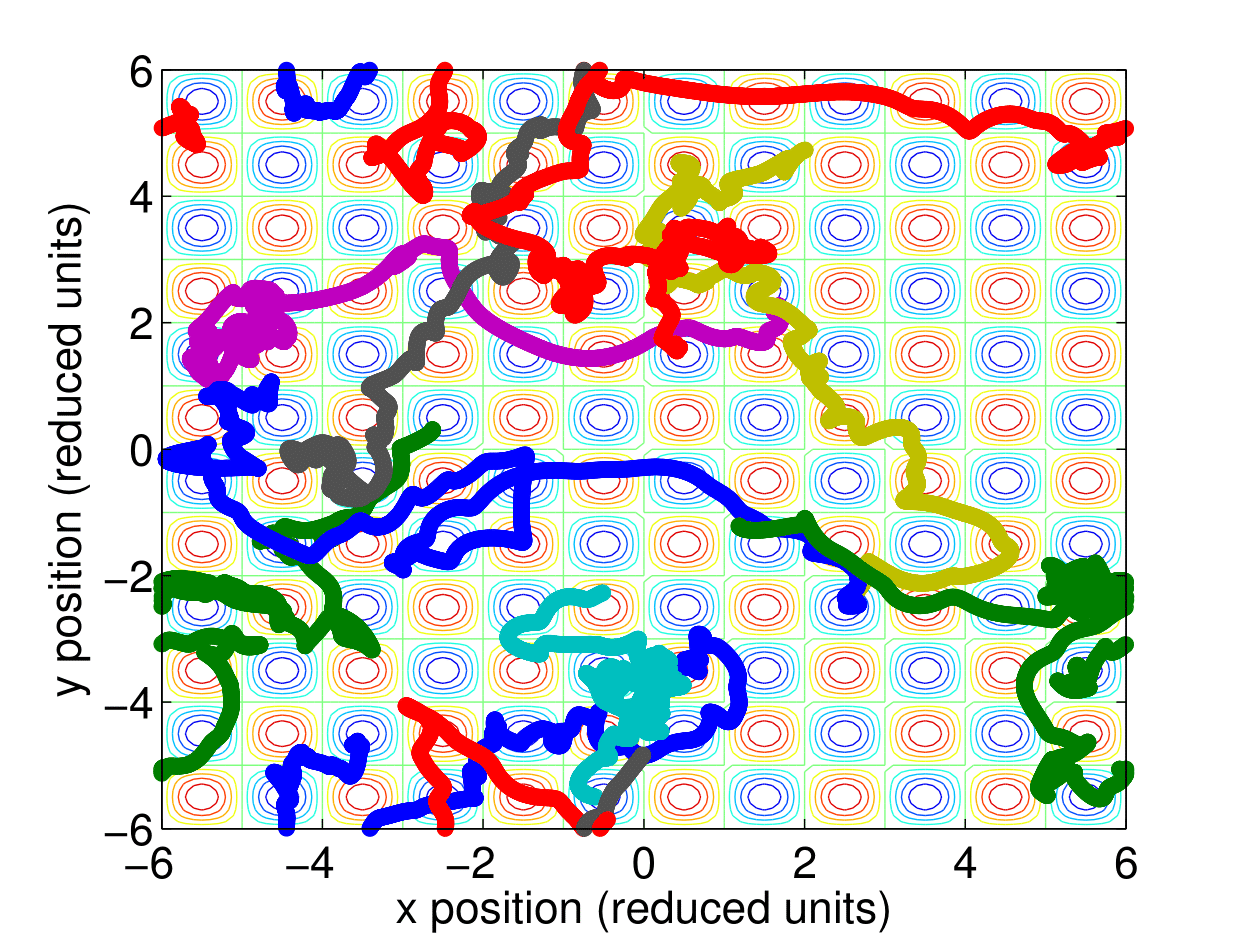
\includegraphics[width=\textwidth]{./figs/ex2-10n-acon0p1-tin0p1.png}
\subcaption{}
\end{minipage}
\hspace{0.02\linewidth}
\begin{minipage}[!htbp]{.5\linewidth}
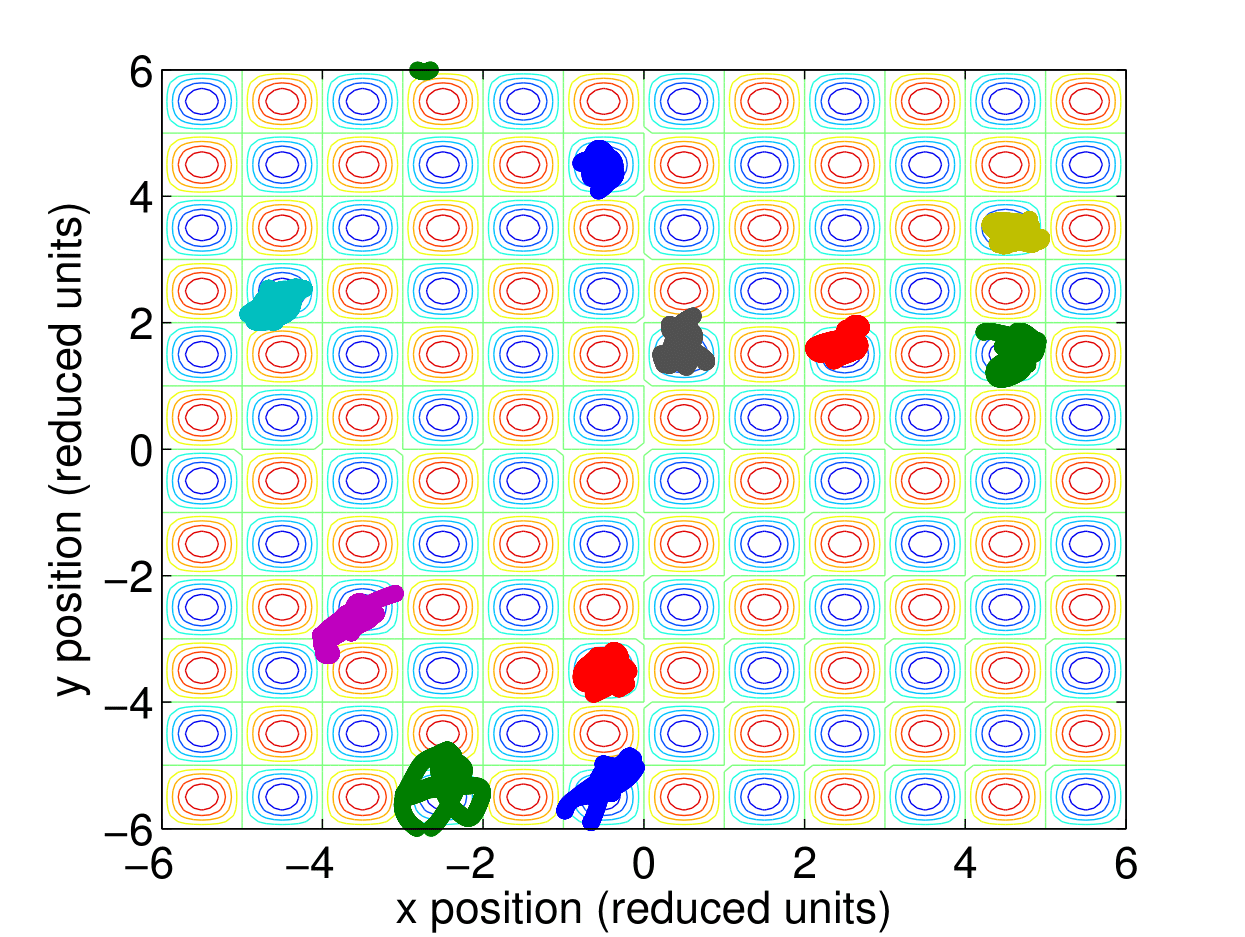
\includegraphics[width=\textwidth]{./figs/ex2-10n-acon1-tin0p1.png}
\subcaption{}
\end{minipage}
\hspace{0.02\linewidth}
\begin{minipage}[!htbp]{.5\linewidth}
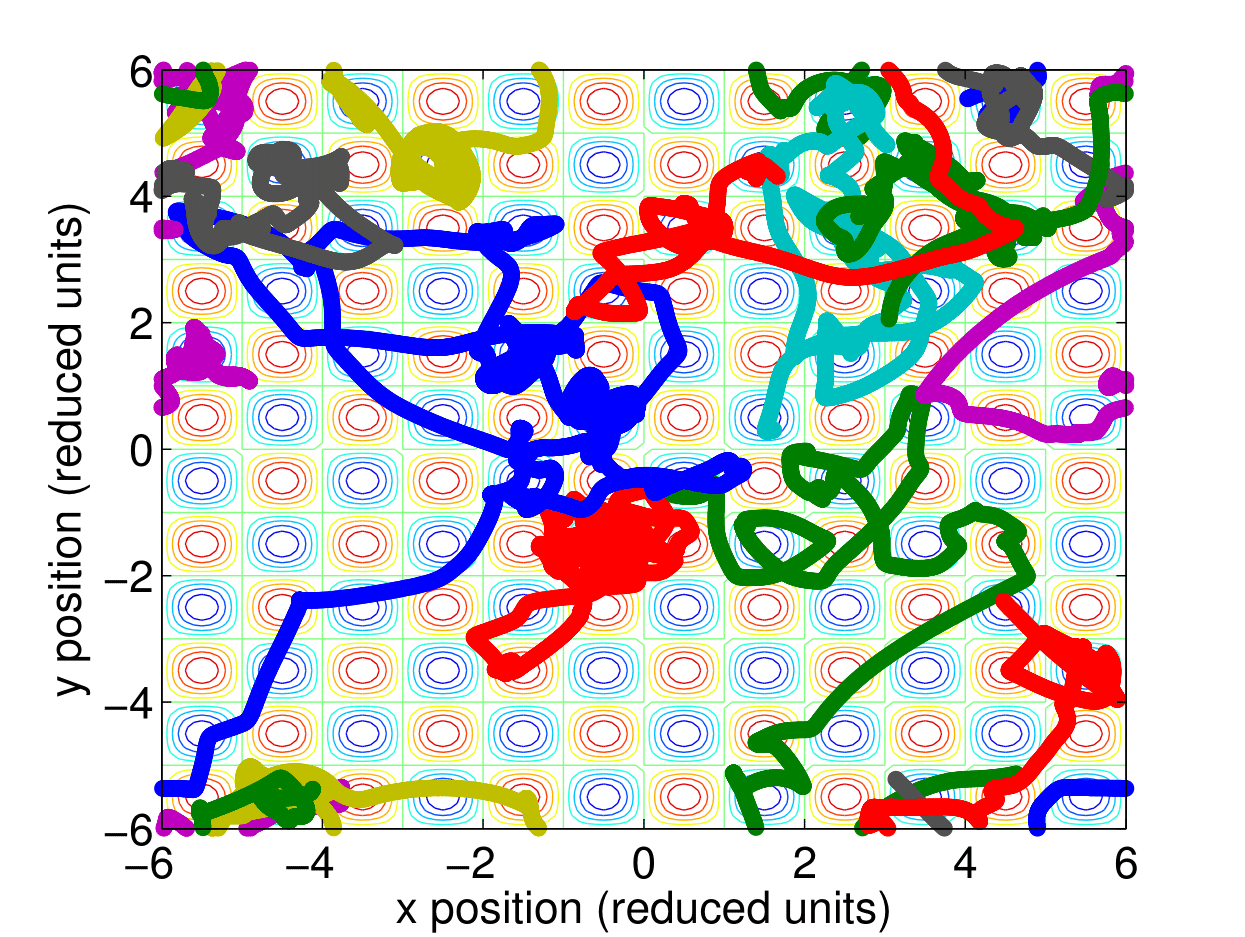
\includegraphics[width=\textwidth]{./figs/ex2-10n-acon1-tin1p2.png}
\subcaption{}
\end{minipage}
\begin{minipage}[!htbp]{.5\linewidth}
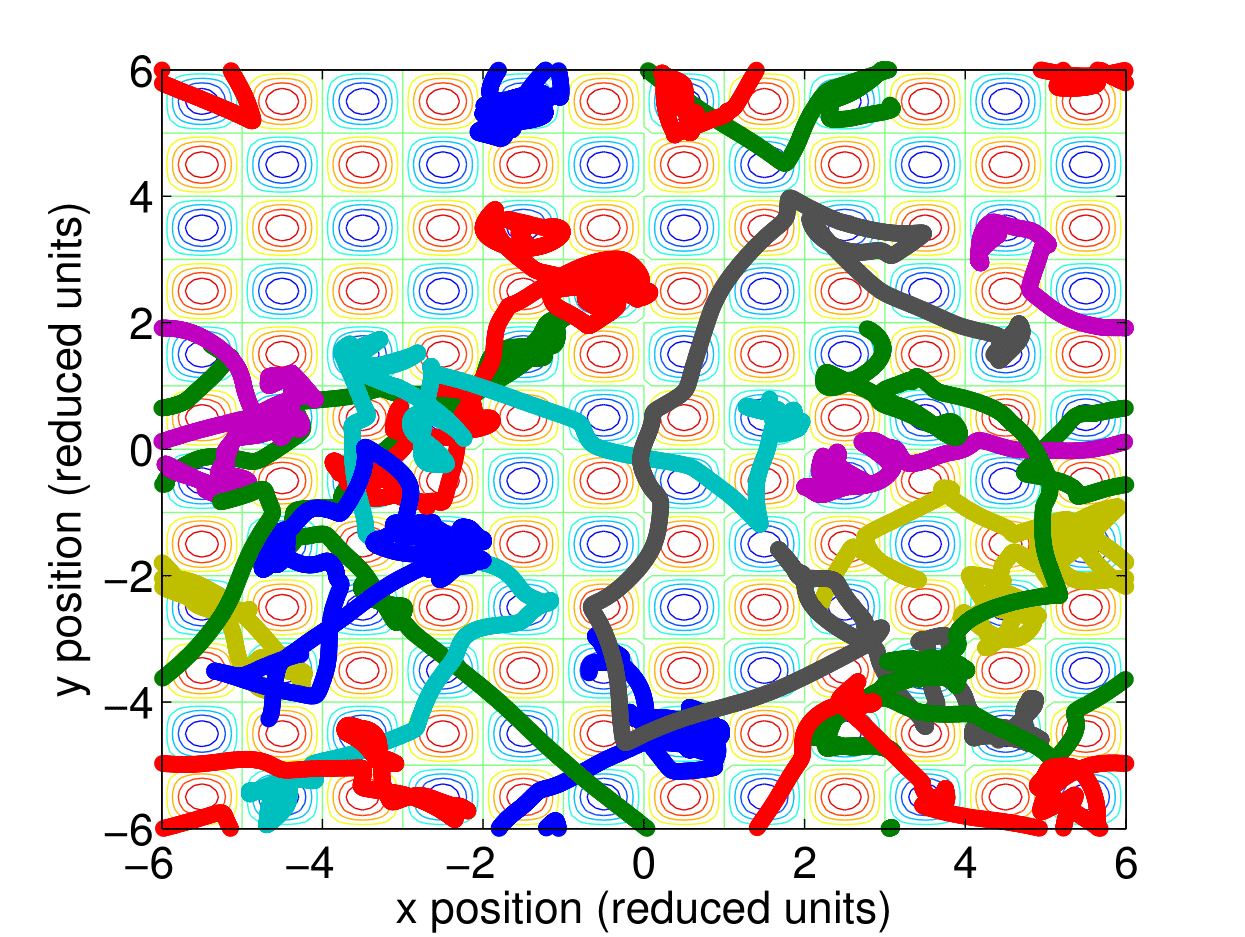
\includegraphics[width=\textwidth]{./figs/ex2-10n-acon1-tin1p5.png}
\subcaption{}
\end{minipage}
\caption{Trajectory for 10 atoms on contour of surface potential for (a) $T_{in} = A = 0.1$, (b) $T_{in} = 0.1, A = 1$, (c) $T_{in} = 1.2, A = 1$ and (d) $T_{in} = 1.5, A = 1$ for 3,000 time steps; all quantities are in reduced units.}
\label{fig:trajmult}
\end{figure}

%--------------------------------------------------------------------------------%
\section{Exercise 4: Bulk FCC- Proper Time Step}

Now we turn to the bulk material. We choose to simulate the parameters of the Ne atom, which has Lennard-Jones parameters $\sigma = 2.74  \AA, \epsilon = 0.0031$ eV and molar mass of 20.1797 g/mol. To get the mass per atom, we divide the molar mass by Avogadro's constant.

a) assuming a time step of $ 5 \cdot 10^{-15}$ s, our predicted time step in reduced units is given by
 
 \begin{equation}
 	dt_{red} = \frac{5 \cdot 10^{-15}}{t_{o}}
 \end{equation}
 
 \noindent where $t_{o}$ is
 
 \begin{equation}
 	t_o = \sqrt{\frac{m_{atom}\sigma^2}{\epsilon}}.
 \end{equation}
 
 From these parameters, we calculate $dt_{calc}$ = 0.0022.
 
 \vspace{5mm}
 b) to calculate the theoretical time step, we use the fact that the period of an atom is $\frac{2\pi}{\omega}$, where $\omega = \sqrt{\frac{k}{m}} $. It can be shown that the spring constant, \textit{k}, is $k = 377\frac{\epsilon}{\sigma^2}$. Assuming 50 time steps per period, we find the theoretical reduced time constant, 
 
\begin{equation}
	dt_{th} = \frac{2\pi}{\sqrt{\frac{k}{m}}}\frac{1}{t_o} = 0.0065,
\end{equation}
 
\noindent which is around three times larger than the one from Lennard-Jones empirical parameters.

%--------------------------------------------------------------------------------%
\section{Exercise 5: Bulk FCC- Confirming proper time step}

For this exercise, we use the following code:

\vspace{5mm}
 \begin{enumerate}
   \item \verb!initLJMD.py!   $\rightarrow$ initialization of positions of \textit{n} atoms; atoms are chosen to sit on \textit{fcc} lattice sites.  
   \item \verb!init3dMB.py!   $\rightarrow$ initialization of velocities for \textit{n} atoms in Maxwell-Boltzmann distribution centered around zero based off of desired temperature input for 3D system.
     \item \verb!fLJsum.py!     $\rightarrow$ contains calculation of forces for 3D Lennard-Jones system; also outputs corresponding potential energy and pressure; uses minimum image convention.
    \item \verb!MDLJ.py!  $\rightarrow$ contains implementation of Verlet Algorithm for 3D bulk system with interaction using Lennard-Jones potential.
    \item \verb!averaging.py!  $\rightarrow$ gives thermodynamic averages of energies, temperature, and pressure.
\end{enumerate}
 \vspace{5mm}

We start from the reduced time step calculated from the empirical Lennard-Jones parameters, dt = 0.0022.
We find it to be a moderate estimate, with fluctuations of around $5 \cdot 10^{-4}$. A larger dt = 0.004 resulted in approximately factor of two larger range of fluctuations. A further reduction of dt = 0.001 does not result in any less fluctuations of the total energy. We therefore keep the original dt = 0.0022, which has fluctuations within the acceptable order of magnitude for numerical variation. Going to smaller time steps may reach fluctuations more aligned with $10^{-4}$ but would require more steps to simulate longer time scales.

Figure \ref{fig:fccdt} illustrates the fluctuations in energy for the various dt time steps tested.

\begin{figure}
\begin{minipage}[!htbp]{.5\linewidth}
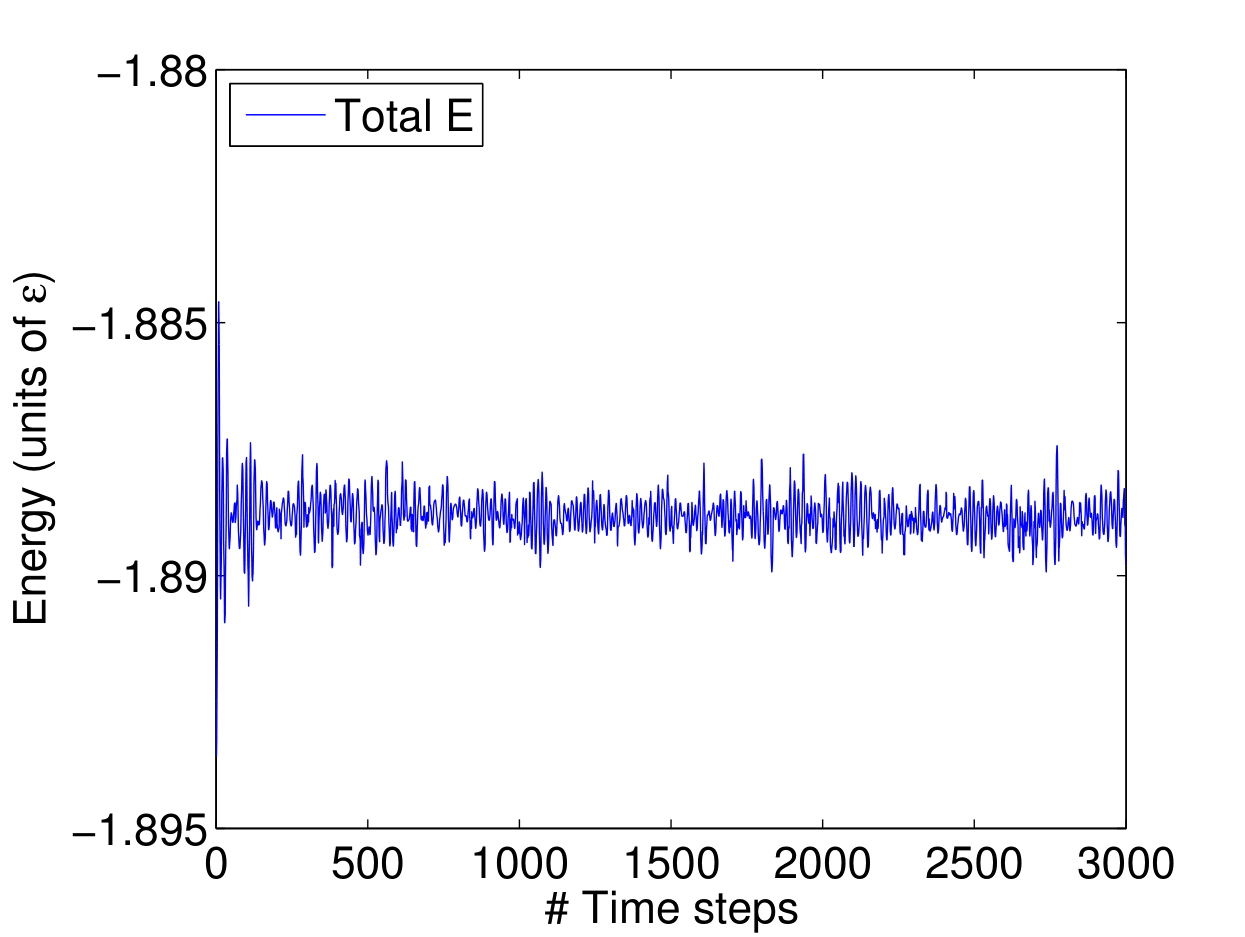
\includegraphics[width=\textwidth]{./figs/ex5-dt=004.png}
\subcaption{}
\end{minipage}
\hspace{0.02\linewidth}
\begin{minipage}[!htbp]{.5\linewidth}
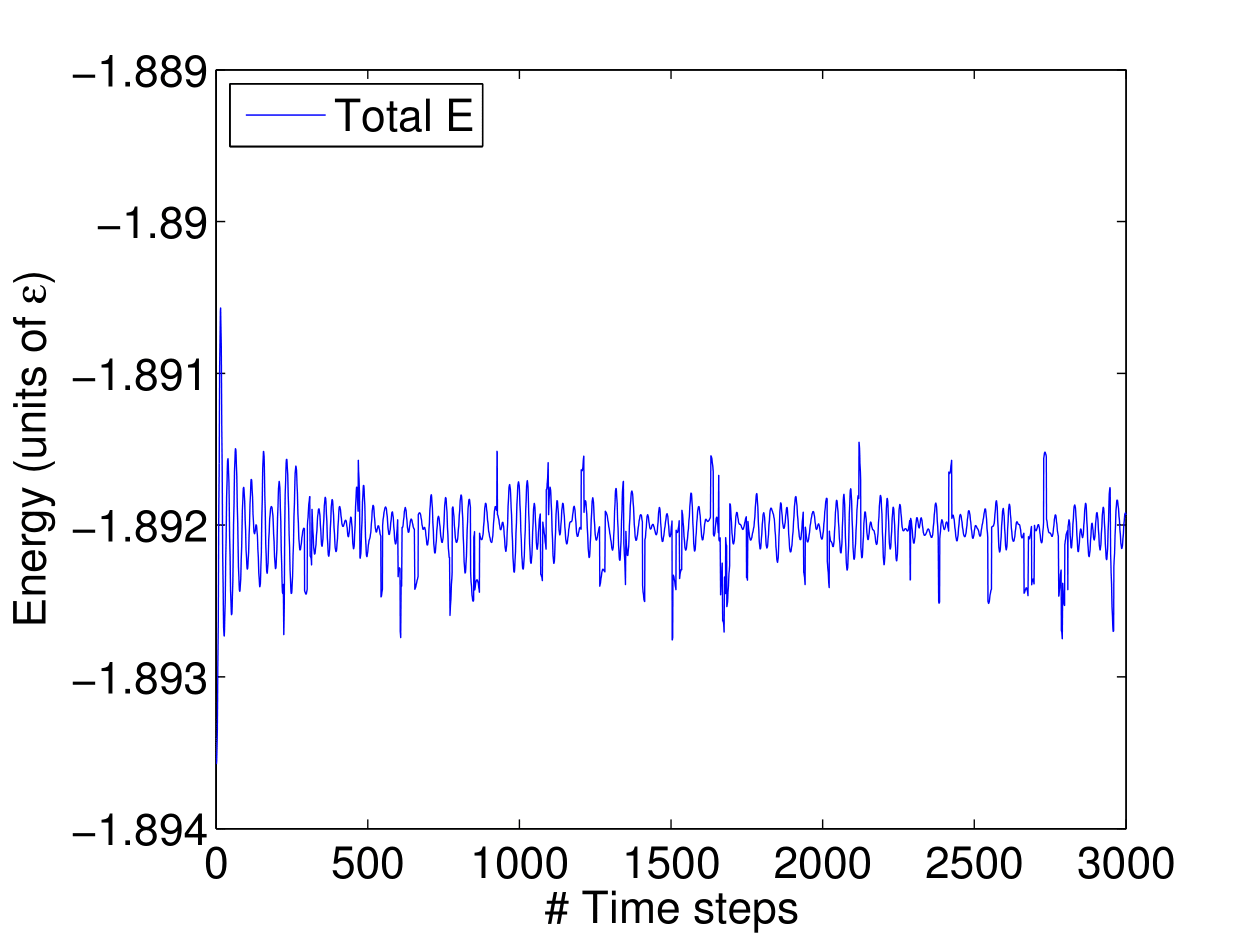
\includegraphics[width=\textwidth]{./figs/ex5-dt=002.png}
\subcaption{}
\end{minipage}
\hspace{0.02\linewidth}
\begin{minipage}[!htbp]{.5\linewidth}
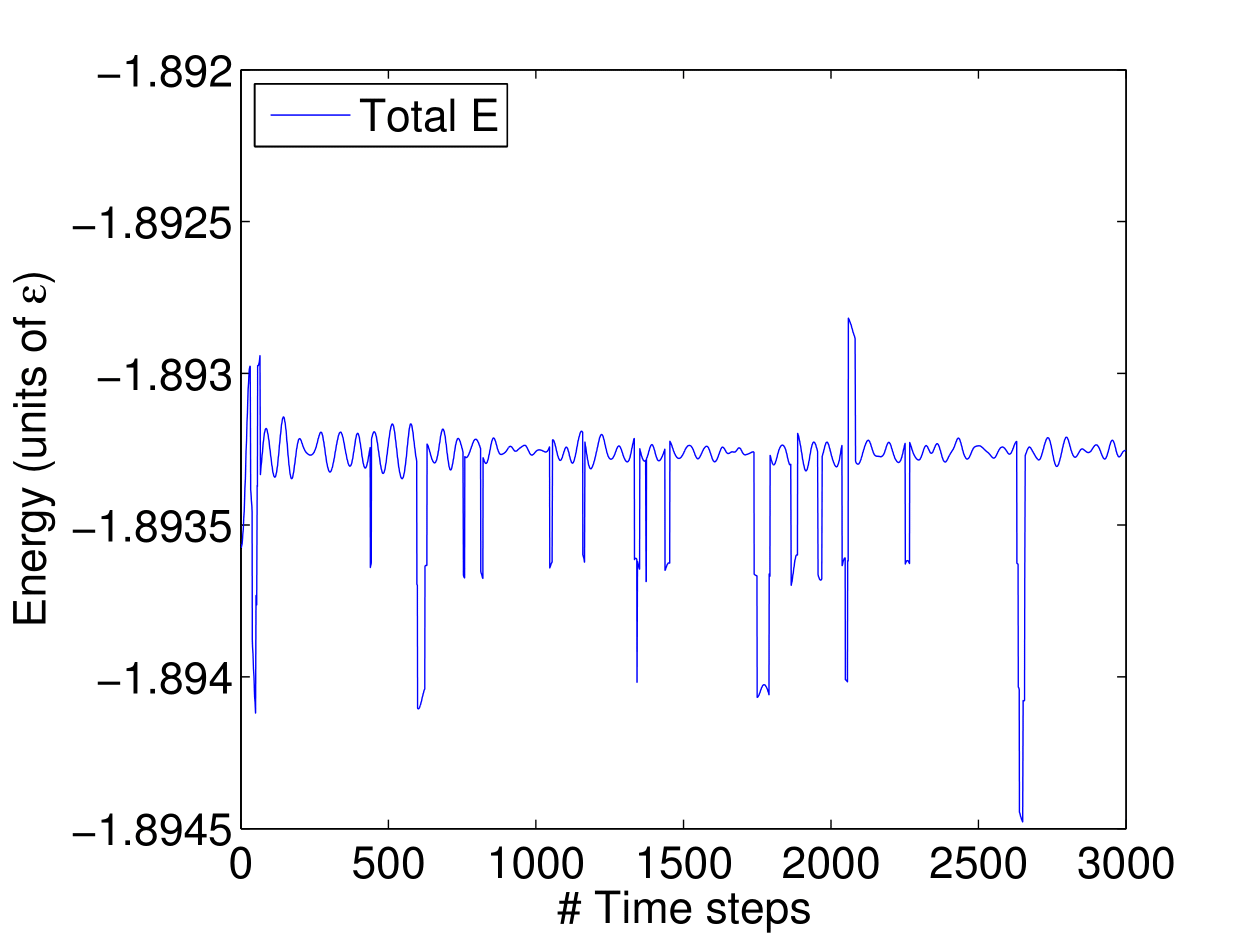
\includegraphics[width=\textwidth]{./figs/ex5-dt=001.png}
\subcaption{}
\end{minipage}
\caption{Convergence of fluctuations in total energy for varying time steps in reduced units, (a) dt = 0.004, (b) dt = 0.002, (c) dt = 0.001}
\label{fig:fccdt}
\end{figure}

%--------------------------------------------------------------------------------%
\section{Exercise 6: Bulk FCC- Solid Phase}

We choose parameters based on the phase diagram for Lennard-Jones materials that result in a solid phase. 
These parameters are 

\begin{verbatim}
reduced density, \rho* = 1.4142
reduced temperature, T* = 1.0
\end{verbatim}

The corresponding equilibration is presented in Figure \ref{fig:fccsolideq}. 

\begin{figure}[htbp]
   \centering
   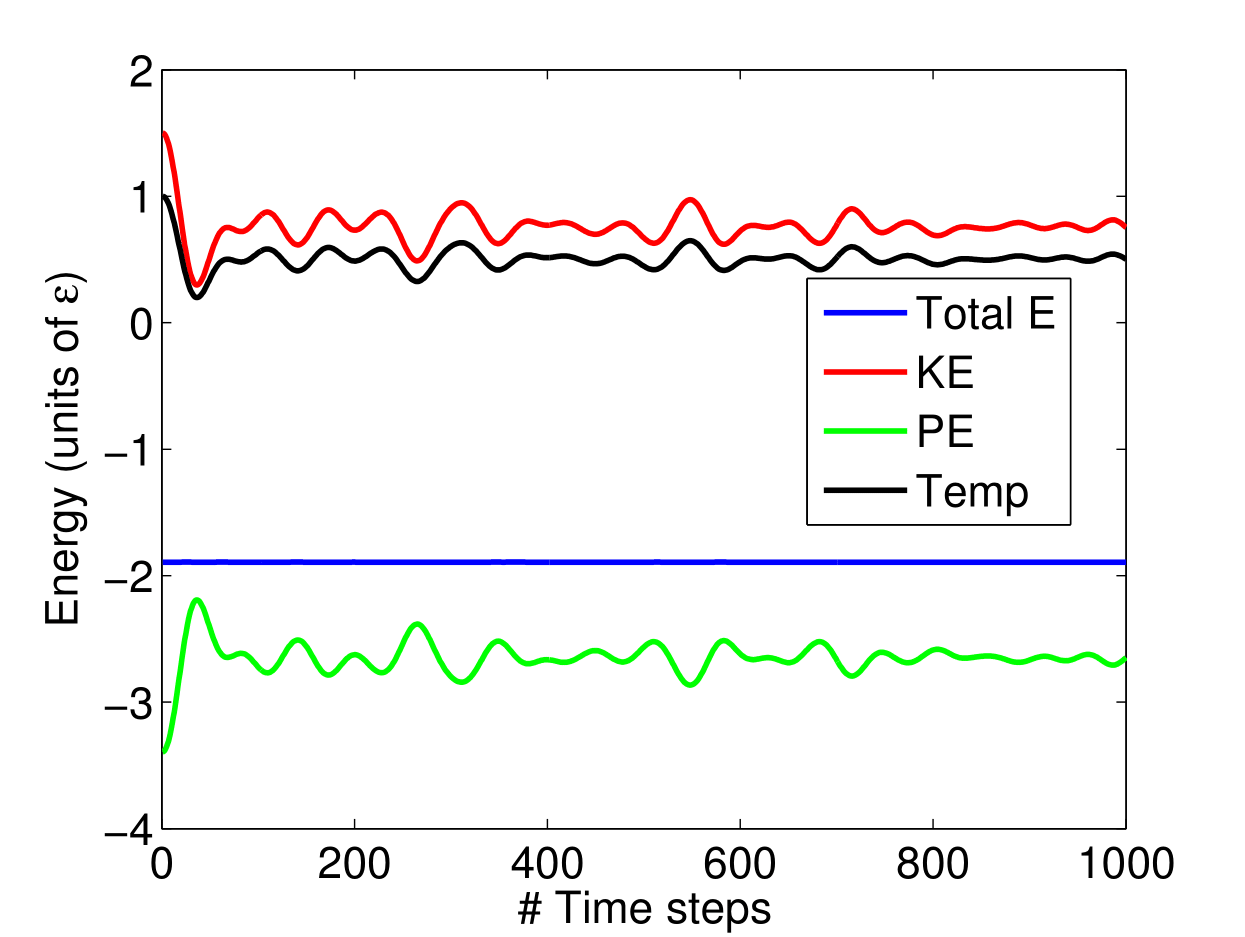
\includegraphics[width=0.8\textwidth]{./figs/ex6-etk.png} % requires the graphicx package
   \caption{Equilibration of solid FCC Lennard-Jones phase for $\rho* = 1.414, t* = 1.0$.}
   \label{fig:fccsolideq}
\end{figure}

It takes around 50 time steps for the run to equilibrate. 

The average of thermodynamic quantities (without the equilibration period) are (in reduced units)

\begin{verbatim}
potential energy, U* = -2.6517
kinetic energy, K*    = 0.7583
energy, E* 	      = -1.8935
temperature, T*      = 0.5055
pressure, P*           = 64.5382
\end{verbatim}

%--------------------------------------------------------------------------------%
\section{Exercise 7: Making the code more efficient}

We rewrite the code in order to separately equilibrate the system, instead of having to for each molecular dynamics simulation.  

We present the code used to invoke this new scheme.

\begin{verbatim}
% for Neon
eps = 0.0031; % eV
sigma = 2.74; % angstroms

nc = 3;  % number repeated cells
tin = 1; % input temperature
% for solid
ao = sigma*2/sqrt(2); % convert from nearest neighbor distance to cubic lattice constant in FCC
n = 4*nc^3; % number of atoms
vol = (ao*nc)^3; % volume, not in reduced units
volred = (ao/sigma*nc)^3;
density = n/volred; % in reduced units
nsteps = 1e3; % number time steps
dt = 0.001; % time step

% equilibration
[n,x,y,z,vx,vy,vz] = initLJMD(nc,tin) ;
[un,kn,en,tn,pn,a,x,y,z,vx,vy,vz]= MDLJi(density,200,dt,n,x,y,z,vx,vy,vz);

% simulation from equilibrated parameters
[un,kn,en,tn,pn,a,x,y,z,vx,vy,vz]= MDLJi(density,nsteps,dt,n,x,y,z,vx,vy,vz);

% averaging time sequence values
xmin = 1; 
xmax = length(un);
[au,ak,ae,at,ap] = averaging(un,kn,en,tn,pn,xmin,xmax)
\end{verbatim}

The modified \verb!MDLKi.py! file has the initialization removed and input/output parameters altered to reflect this.

A set of averages with this newly modified molecular dynamics simulation. 

\begin{verbatim}
potential energy =  -2.6496
kinetic energy  = 0.7570
total energy =  -1.8926
temperature = 0.5046
pressure = 64.5482
\end{verbatim}

These averages are not drastically different from the previously calculated averages and are not outside the range of numerical variation observed in general. Thus, the number of steps for these runs (i.e., 1000) allowed to run are sufficiently long enough to avoid the issue of drift in calculations.

%--------------------------------------------------------------------------------%
\section{Exercise 8: Bulk FCC- Liquid phase}

We repeat the analysis as we did for solid phase Lennard-Jonesium for parameters that simulates liquid Lennard-Jonesium. For these runs, based on the phase diagram provided, we choose $\rho* = 0.4, T* = 1$. Figure \ref{fig:liq} presents the evolution of the kinetic, potential, and total energy over time steps.

\begin{figure}[htbp]
   \centering
   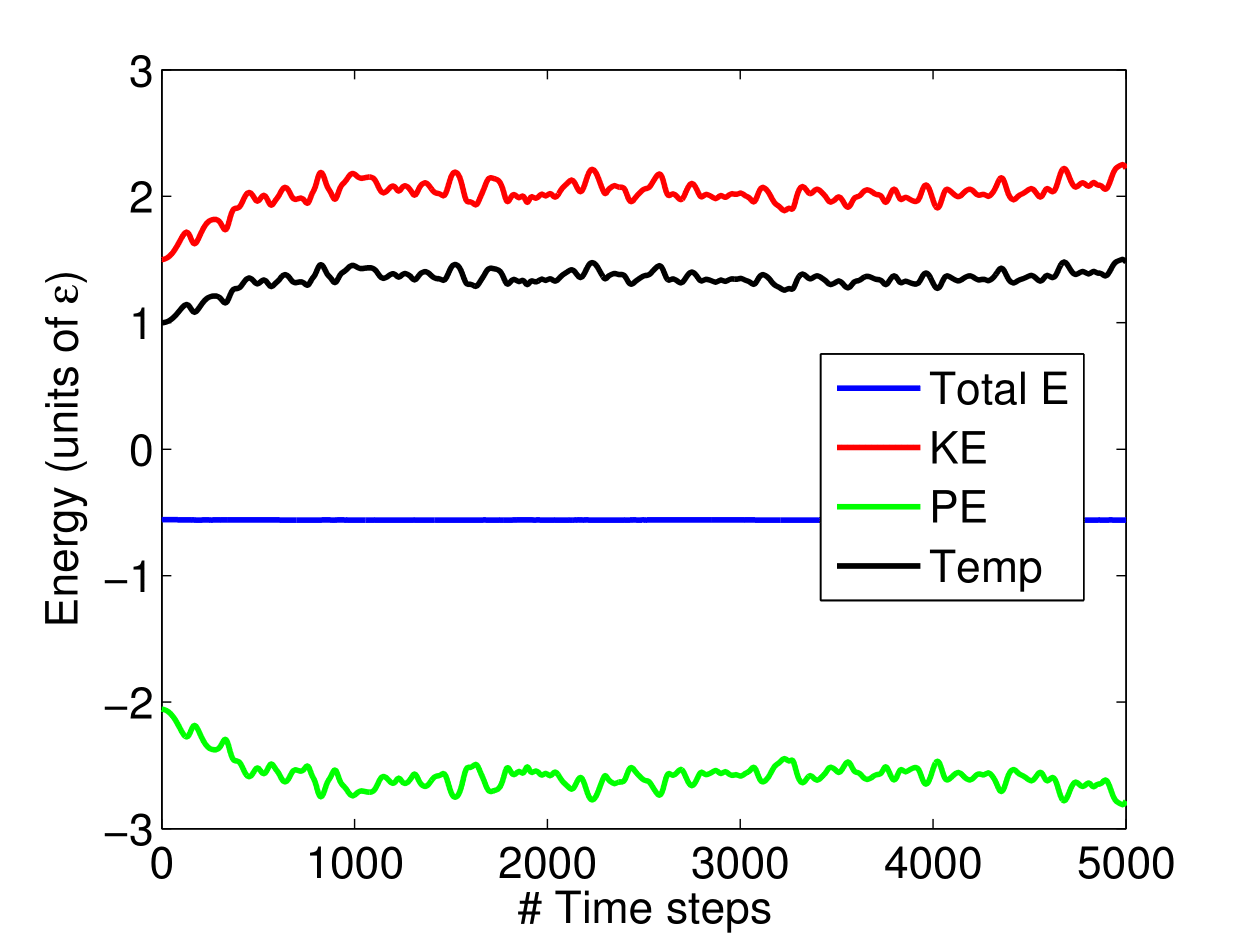
\includegraphics{./figs/ex8-etk.png} % requires the graphicx package
   \caption{Tracking relation between kinetic, potential, and total energy for liquid phase of bulk FCC Lennard-Jonesium}
   \label{fig:liq}
\end{figure}

Equilibration takes around 1000 time steps before equilibration is reached.

Below we present the average values of thermodynamic quantities for the liquid phase over 5000 time steps for the choice of $\rho* = 0.4, T* = 1$ for the code with initialization and equilibration included in the molecular dynamics simulation (i.e., using \verb!MDLJ.py!, not \verb!MDLJi.py!).

\begin{verbatim}
U* 	= -2.5835
K*    = 2.0234
E*    = -0.5601
T*    = 1.3489
P*    = 0.2161
\end{verbatim}

Using instead \verb!MDLJi.py! for comparison, we find the following average values for 5000 time steps (excluding equilibration), 

\begin{verbatim}
U* 	= -2.6144
K*    = 2.0539
E*    = -0.5606
T*    = 1.3693
P*    = 0.2262
\end{verbatim}

As with the solid phase, the differences between the two methods of initialization and equilibration are similar to the fluctuations observed between each molecular dynamics run and are on the order of $10^{-2}$ in reduced units for the time step size chosen. Drift is similar magnitude to the solid phase and to the variation that occurs between molecular dynamics runs of the same method. Longer runs may reduce the drift in both the case of the solid and liquid, but the length of runs presented presents a distinction enough between the solid and liquid phases.

%--------------------------------------------------------------------------------%
\section{Exercise 9: Calculating thermodynamic capacities}

Using the time series data already available, we are able to calculate fluctuations in quantities of thermodynamic capacities. We present the variance of the various thermodynamic quantities so far for the solid and liquid phase. In addition to using the files mentioned in Exercise 5, we also use the file \verb!variance.py! for calculating the variance.

We also include the averages for the same run for comparison.

For the solid phase, using a density $\rho* = 1.414$ and T* = 1 for 5000 time steps, we find the following

\begin{verbatim}
U* 			= -2.6539
K*			= 0.7549
E* 			= -1.8990
T*			= 0.5032
p* 			= 64.4770
\end{verbatim}

$\sigma_{U}^*$ 	=  -0.0029,
$\sigma_{K}^*$ 	=  -0.0029,
$\sigma_{E}^*$	= -1.0232e-07,
$\sigma_{T}^*$	= -0.0013,
$\sigma_{p}^*$ 	= -0.0857,



For the liquid phase, using a density $\rho* = 0.4$ and T* = 1 for 5000 time steps (excluding equilibration), we find the following

\begin{verbatim}
U* 			= -2.6417
K*			= 2.0797
E* 			= -0.5620
T*			=  1.3865
p* 			=  0.2321
\end{verbatim}

$\sigma_{U}^*$ 	=  -0.0042,
$\sigma_{K}^*$ 	=  -0.0042,
$\sigma_{E}^*$	= -4.7321e-07,
$\sigma_{T}^*$	= -0.0019,
$\sigma_{p}^*$ 	= -0.0301,


As seen from the above data, the liquid phase undergoes more fluctuations in its thermodynamic parameters than the solid phase. This is consistent with the picture of thermal vibrations between a solid and liquid phase. Additionally, the liquid phase is less energetically favorable than the solid ($E_{l}* > E_{s}*$), and consequently have species with larger kinetic energy, also consistent with the intuitive picture of atomic motion in a liquid versus solid phase.

%--------------------------------------------------------------------------------%
\section{Exercise 10: Radial Distribution Function}

We can learn more about the structure of the phases we simulated in previous exercises using the radial distribution function, which provides information on the probability and atom is located a distance \textit{r} away from a reference atom. For crystalline solids, the radial distribution function is composed of defined peaks where as in less structured phases, such as liquid, the curve is more continuous and eventually asymptotes to unity.

We implement the calculation of the radial distribution function in the simulation for molecular dynamics, specifically when forces are calculated.

\vspace{5mm}
 \begin{enumerate}
   \item \verb!initLJMD.py!   $\rightarrow$ initialization of positions of \textit{n} atoms; atoms are chosen to sit on \textit{fcc} lattice sites.  
   \item \verb!init3dMB.py!   $\rightarrow$ initialization of velocities for \textit{n} atoms in Maxwell-Boltzmann distribution centered around zero based off of desired temperature input for 3D system.
     \item \verb!fLJsumg.py!     $\rightarrow$ contains calculation of forces for 3D Lennard-Jones system that includes calculation of the radial distribution function
    \item \verb!MDLJg.py!  $\rightarrow$ contains implementation of Verlet Algorithm for 3D bulk system with interaction using Lennard-Jones potential and includes calculation of radial distribution function.
\end{enumerate}
\vspace{5mm}
 
Figure \ref{fig:g(r)} present the radial distribution function for the solid and liquid phase of the simulation cell size chosen, using 50 bins and 5000 time steps at T* = 1. The plots cutoff at the size of the simulation cell, which is chosen to be 3 repeated unit cells in each direction.

\begin{figure}
\begin{minipage}[!htbp]{.5\linewidth}
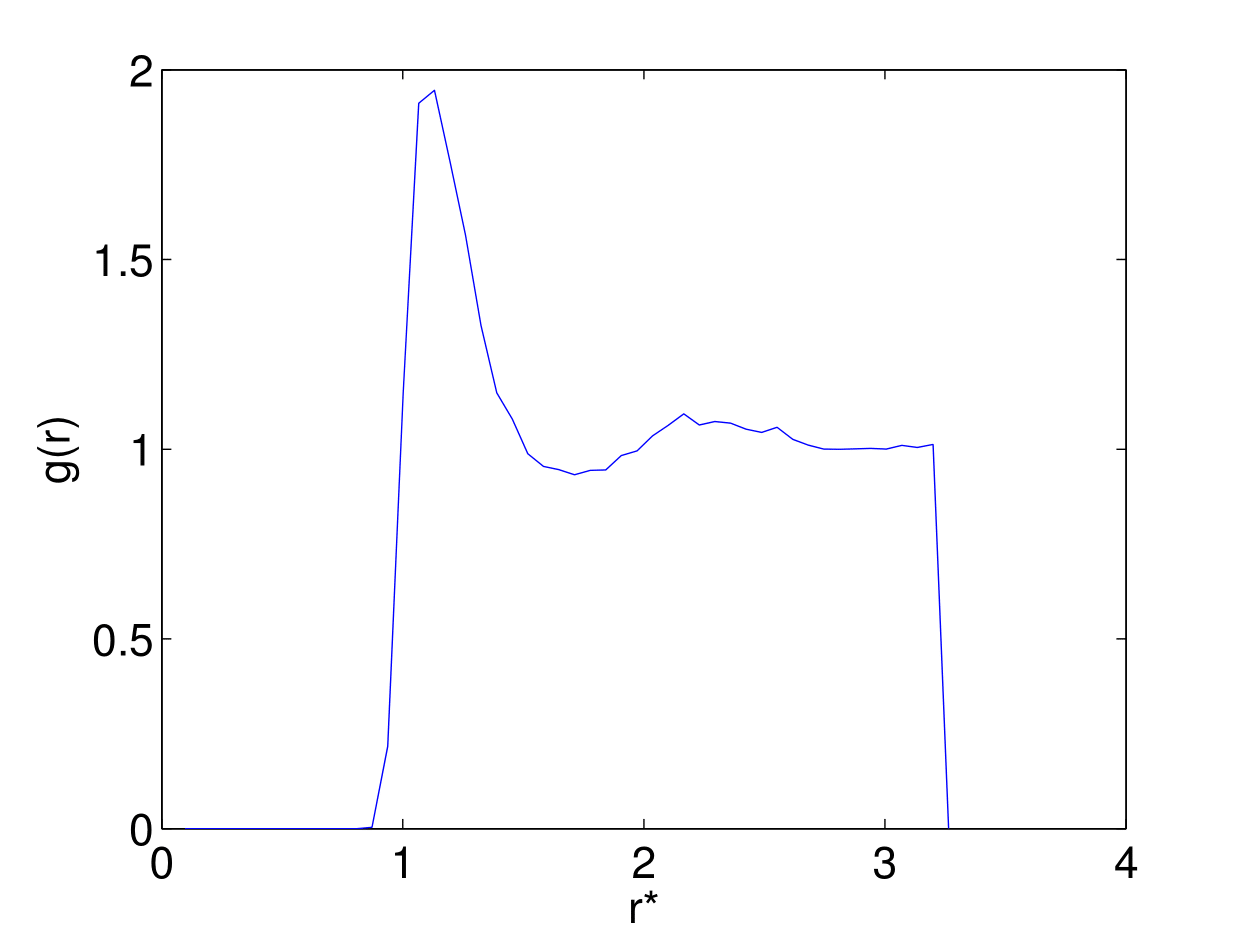
\includegraphics[width=\textwidth]{./figs/ex10-gr-liq.png}
\subcaption{}
\end{minipage}
\hspace{0.02\linewidth}
\begin{minipage}[!htbp]{.5\linewidth}
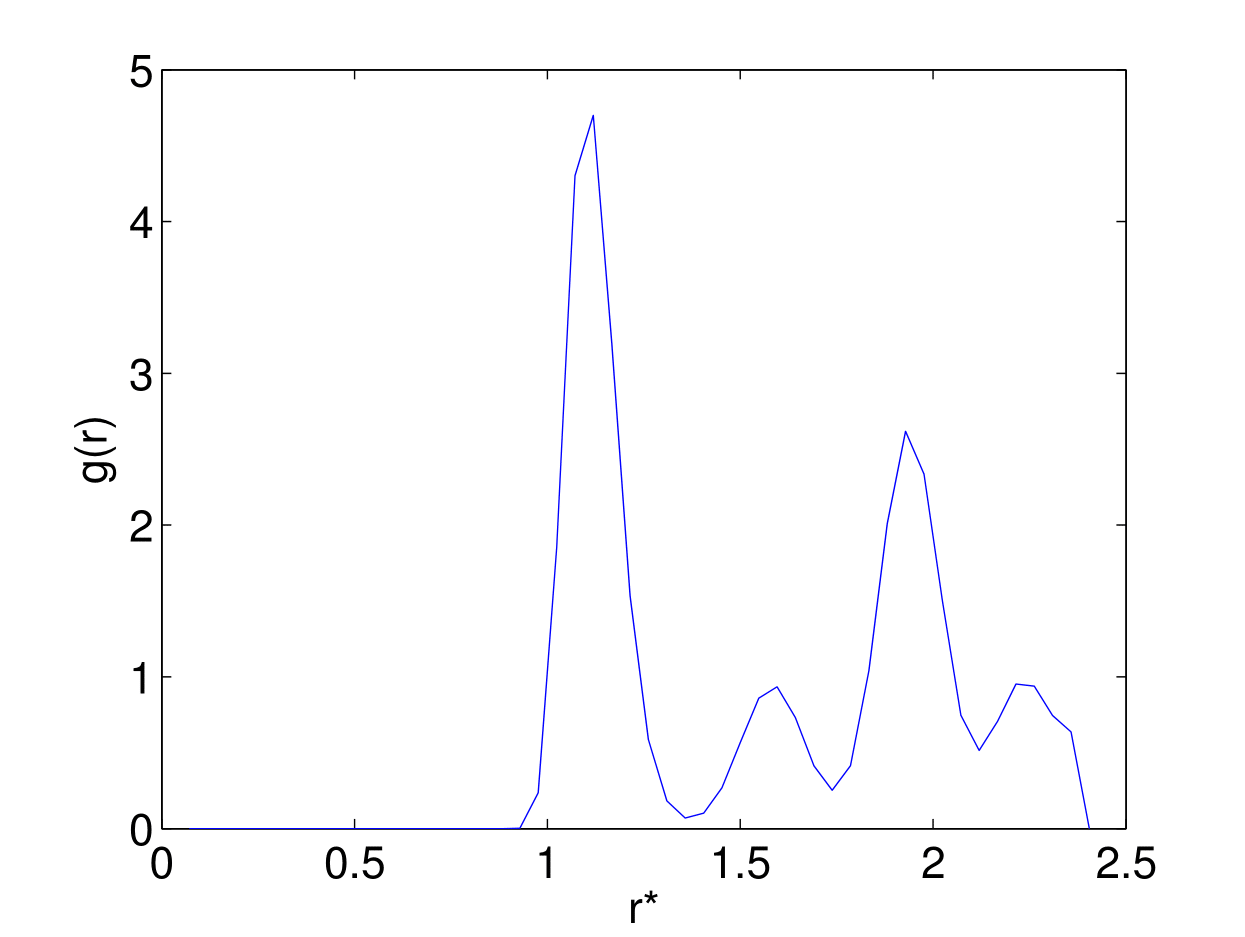
\includegraphics[width=\textwidth]{./figs/ex10-gr-sol-rho1.png}
\subcaption{}
\end{minipage}
\caption{Radial distribution function for Lennard-Jonesium in (a) liquid phase, $\rho*$ = 0.4 and  (b) solid phase, $\rho* = 1$ at T* = 1}
\label{fig:g(r)}
\end{figure}

The radial distribution function gives clear indication of the phase the material is in for the parameters tested.

%--------------------------------------------------------------------------------%
\section{Exercise 11: Structural Order Parameter}

We may also infer additional information from the structural order parameter. The structure order parameter for \textit{N} atoms is defined as

\begin{equation}
 	\rho(\vec{k}) = \frac{1}{N}  \sum\limits_{i=1}^N cos(\vec{k}\cdot \vec{r_i})
\end{equation}

For an \textit{ccc} lattice, $\vec{k} = \frac{2\pi}{a_{fcc}}(-1,1,-1)$, a reciprocal lattice vector, where $a_{fcc}$ is the lattice constant of the unit cell, \textit{not} the simulation cell size. However, $\vec{r_i}$ are the position coordinates scaled to the simulation cell size. A perfectly \textit{fcc} lattice will have $\rho(\vec{k}) = 1$, where as a non-\textit{fcc} phase will have $\rho(\vec{k}) = 0$. What this other phase is may be a liquid or a different crystalline phase.

Figure \ref{fig:rho} presents the structural order parameters for the solid and liquid phases including equilibration to see the evolution of the structure factor for 5000 time steps.

\begin{figure}
\begin{minipage}[!htbp]{.5\linewidth}
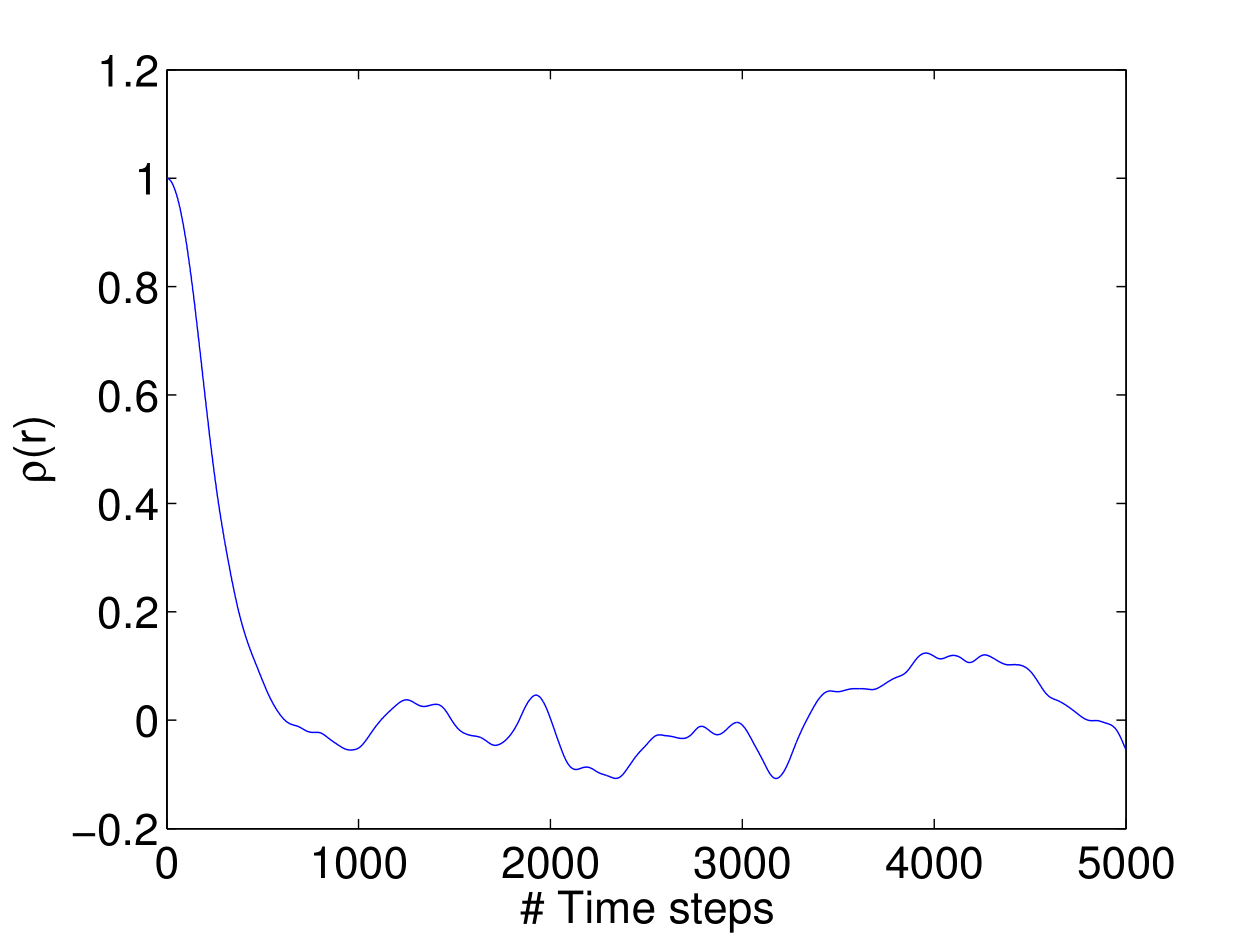
\includegraphics[width=\textwidth]{./figs/ex11-rho-liq.png}
\subcaption{}
\end{minipage}
\begin{minipage}[!htbp]{.5\linewidth}
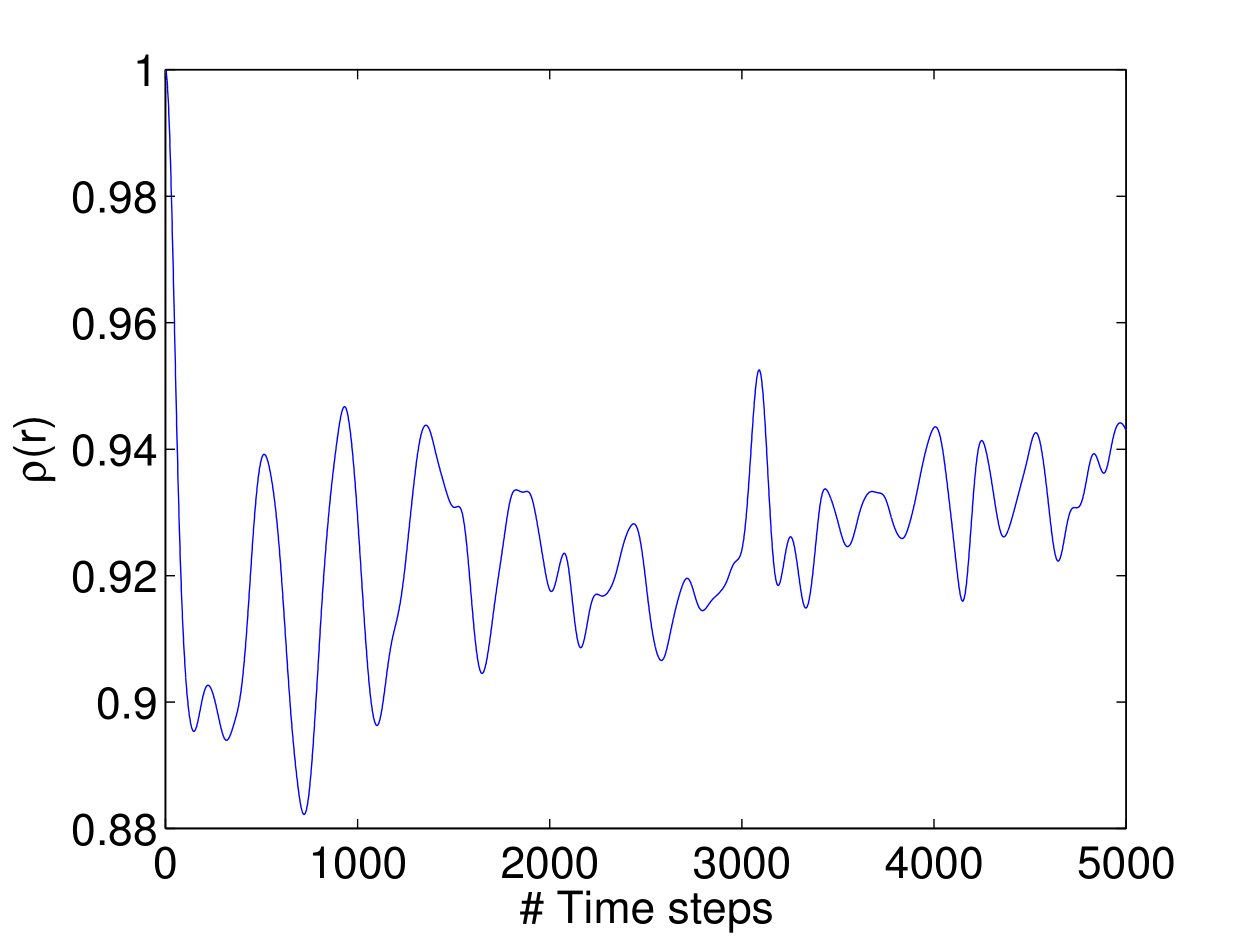
\includegraphics[width=\textwidth]{./figs/ex11-rho-sol.png}
\subcaption{}
\end{minipage}
\caption{Structural order parameter for Lennard-Jonesium in (a) liquid phase, $\rho*$ = 0.4 and  (b) solid phase, $\rho* = 1$ at T* = 1}
\label{fig:rho}
\end{figure}

As seen in Figure \ref{fig:rho}, both the liquid and solid phases begin as \textit{fcc} structures with $\rho(\vec{k}) = 1$. As the liquid equilibrates, $\rho(\vec{k})$ drops and oscillates around zero, indicating that it has lost its original \textit{fcc} ordering. In contrast, the solid phase retains a fairly consistent $\rho(\vec{k}) ~ 1 $, indicating it retained its \textit{fcc} structure. It agrees with what we expect and what is observed in Exercise 10. 

The structural order parameter provides additional quantitative information to the extent that a phase retains its starting structure, and is easier to visualize as a function time. It is also specific to a particular ordering, depending on the choice of $\vec{k}$, and so provides crystal system specific information that is hidden in the radial distribution function. 


%--------------------------------------------------------------------------------%
\section{Exercise 12: Velocity Autocorrelation Function}

We conclude with a calculation of the velocity autocorrelation function that is an average over all particles for the liquid and solid phase. We implement the velocity autocorrelation function in the less sophisticated way, so sizable fluctuations are expected.The velocity autocorrelation function is defined as 

\begin{equation}
	c_{vv} = \frac{m}{3 k_b T} < \vec{v}(t) \cdot \vec{v}(0) >
\end{equation}

The corresponding velocity autocorrelation as a function of time step for the liquid and solid phases is plotted in Figure \ref{fig:vac}.

\begin{figure}
\begin{minipage}[!htbp]{.5\linewidth}
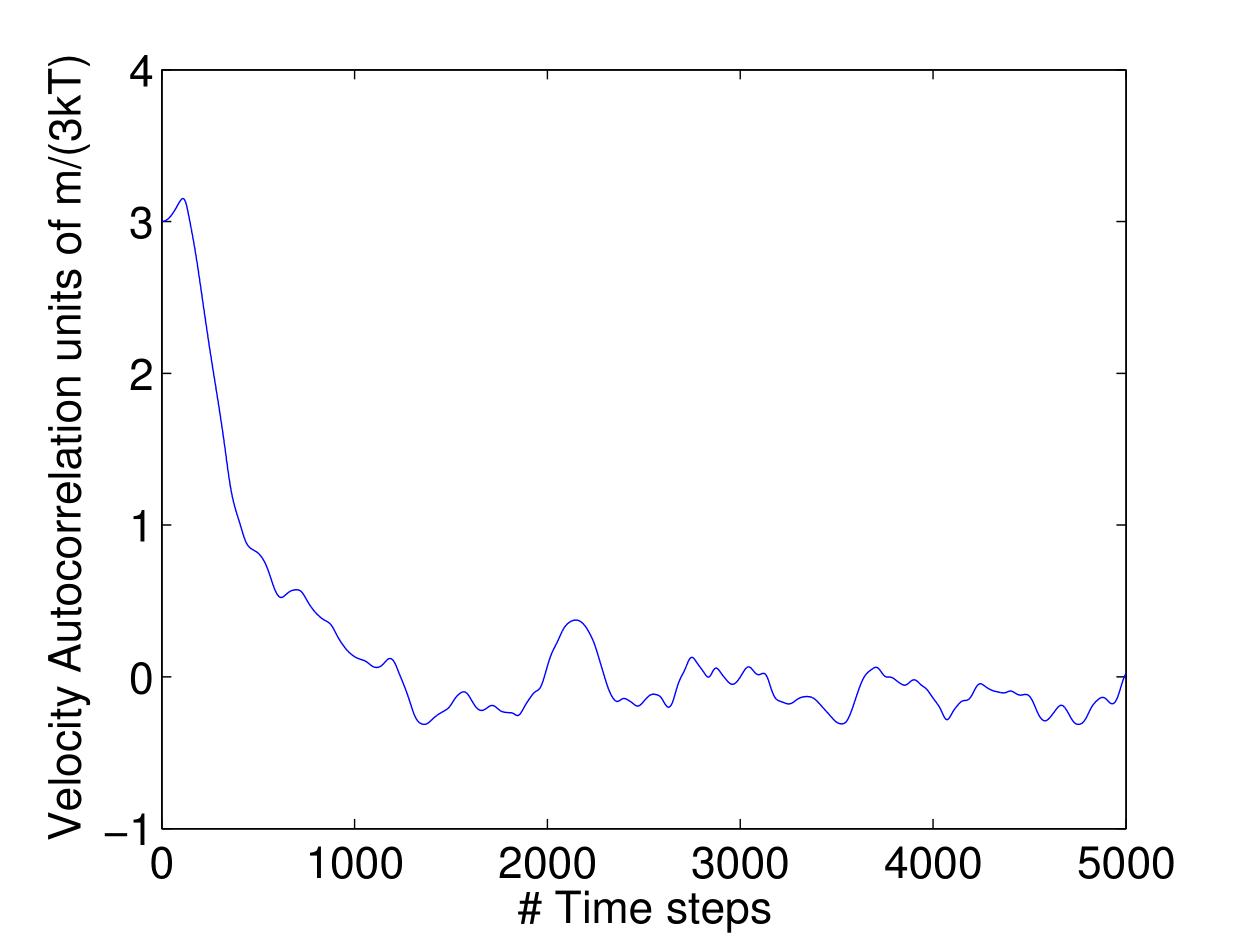
\includegraphics[width=\textwidth]{./figs/ex12-vac-liq.png}
\subcaption{}
\end{minipage}
\begin{minipage}[!htbp]{.5\linewidth}
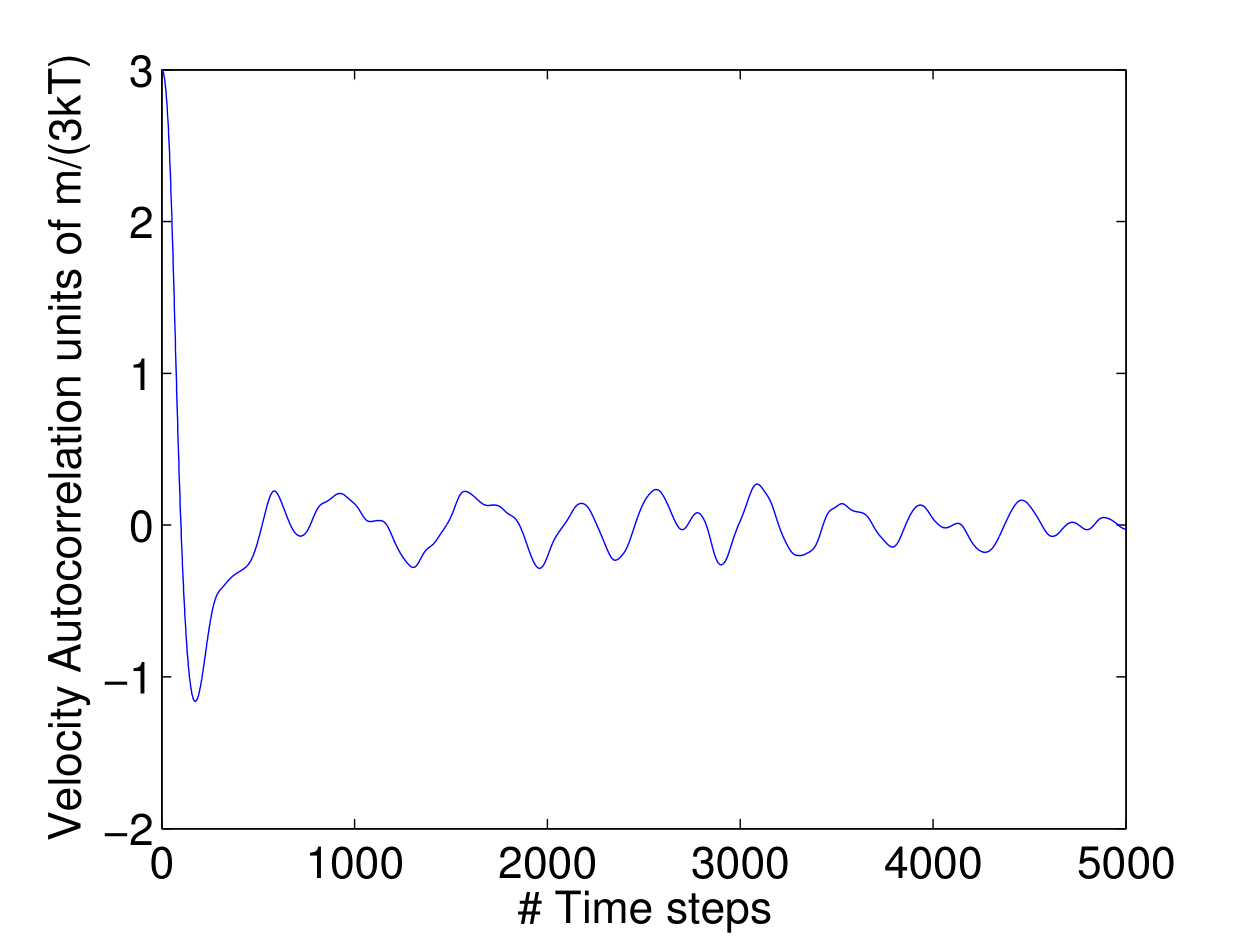
\includegraphics[width=\textwidth]{./figs/ex12-vac-sol.png}
\subcaption{}
\end{minipage}
\caption{Velocity autocorrelation function for Lennard-Jonesium in (a) liquid phase, $\rho*$ = 0.4 and  (b) solid phase, $\rho* = 1$ at T* = 1}
\label{fig:vac}
\end{figure}

Autocorrelation functions measure the extent of correlation between two variables, specifically between two instances in time. With longer runs, the autocorrelation function is expected to decay to zero. This is indeed what is observed for both the liquid and solid phase. However, for this liquid phase, this decay is slow. This is rather unexpected as for a liquid, one would expect the many random collisions would cause a faster decay of correlation between velocities. The long tail decay that is observed suggests more complicated behavior. For the solid phase, one observes a negative autocorrelation at the onset of the simulation, which is behavior typically observed for denser systems at lower temperatures, corresponding to collisions with neighboring atoms that are like backscattering.

\end{document}
